\documentclass{puthesis}
\usepackage{latexsym}
\usepackage{graphicx}
\usepackage{url}       % SB
\usepackage{algorithmic}
\usepackage{algorithm}
\usepackage{times}
\usepackage{xcolor}
\usepackage{textcomp}
\usepackage{mathpartir}
\usepackage{semantic}
\usepackage{listings}
\usepackage{lstlangcoq}
\usepackage{caption}
\usepackage{stmaryrd}
\usepackage{placeins}
\renewcommand{\lstlistingname}{Figure}
\newcommand{\PROP}{\mbox{\small PROP}}
\newcommand{\LOCAL}{\mbox{\small LOCAL}}
\newcommand{\SEP}{\mbox{\small SEP}}
\newcommand{\later}{\triangleright}
\newcommand{\wand}{\mathrel{-\hspace{-.7ex}*}}
\newcommand{\triple}[3]{\{#1\}\,#2\,\{#3\}}
\newcommand{\name}{Verified Software Toolchain}
\newcommand{\defeq}{=_{\mathrm{def}}}




\lstset{language=Coq,alsoletter=_,basicstyle=\sffamily,mathescape=true,columns=fullflexible}



\author{Josiah Dodds}
\adviser{Andrew Appel}
\title{Computation Improves Interactive Symbolic Execution}
\abstract{
We are surrounded by more and more critical software every day. This
is the software that we trust with our lives and happiness; software
whose failure comes with an extraordinary cost. Much of this software
is written in C, a common language to use when performance is
critical. Unfortunately, the C programming language is less convenient
for writing \emph{correct} programs. It contains a number of pitfalls
that make it difficult to write correct programs, and a number of
these pitfalls also make it difficult to show that an existing program
is correct. 

Verifiable C is an expressive Hoare logic (higher-order
impredicative concurrent separation logic) for proving functional
correctness of C programs.  The program logic is foundational---it
is proved sound in Coq w.r.t. the operational semantics of CompCert
Clight.  Users apply the program logic to C programs using
semiautomated tactics in Coq, but
these tactics are very slow.

\qquad This thesis shows how to make an efficient (yet still
foundational) symbolic executor based on this separation logic by
using computational reflection in several different ways.  Our
execution engine is able to interact gracefully with the user by
reflecting application-specific proof goals back to the user for
interactive proof---necessary in functional correctness proofs where
there is almost always domain-specific reasoning to be done.  We use
our ``mostly sound'' type system, computationally efficient finite-map
data structures, and the MirrorCore framework for computationally
reflected logics.  Measurements show a 40$\times$
performance improvement.}
\acknowledgements{Thank you very much.}
\dedication{To myself.}



\begin{document}



\chapter{Introduction}

The C programming language is one of the most commonly used languages
for writing critical software. C is often used for operating systems,
embedded systems, and cryptography, as well as countless libraries
that need to have high performance while being compatible with as many
languages and systems as possible. The world depends on more systems
every day, and many of those systems have C code at their core.

In general, the code we depend on works well, and there is plenty of
noncritical code that can fail without causing harm but when critical
code fails, it can be catastrophic. Space projects that cost hundreds
of millions of dollars have failed due to problems with software
\cite{polarlander, marsorbit}, radiation device software has caused
overdoses in cancer patients\cite{therac}, and millions of cars have
been recalled to fix software bugs\cite{toyotarecall}. Those scenarios
are only caused by bugs; far more systems can fail when a malicious
user attacks them. As an example, a brand of refrigerators was found
to have been taken over to send spam e-mail \cite{fridgenet}.

To believe that a C program will run correctly we must first believe a
number of other things. There are a number of components that we will
need to be able to \emph{trust} in order to trust our C program. We need
to fully understand the program itself, and believe that it will do
what we want it to. We also need to believe that when
the C code is translated into machine language, the generated machine
language has the same behavior as the original program. Finally we
need to believe that the machine executing the machine language is
doing the correct thing. We call the collection of things we must
trust the \emph{trusted computing base}. In general, the larger the
trusted computing base is, the harder it is to be confident that the
program is correct.

The need for trust follows a chain. It starts with the C program at
the top, the most human understandable part of the chain, and moves
down to the actual execution of the machine. In order to make the
trusted computing base as small as possible, we must maximize our
confidence in every step of the process\footnote{If we cannot trust
  the C code or the C compiler, we can review or verify the
  assembly-language program; this approach is often used in practice,
  but it is difficult and tedious.}.

Proof assistants are tools for stating theorems, and then writing and
checking proofs of those theorems. If you want to believe a pen and
paper mathematical proof you first need to understand the statement of
the proof, which is open to ambiguities based on (often unstated)
assumptions made by the writer, and then believe every single step of
the proof itself, even steps where the proof author says something
vague like ``clearly'' or ``obviously''. This can be an enormous
burden on the person that needs to understand how the proof was done;
new proofs can use new techniques that are impenetrable to anyone but
experts in the specific domain of the proof. This is a real problem,
because often the theorem proved is useful to many people even if the
proof itself is difficult for them to understand. If you want to use a
pen and paper proof that you can't understand, you must trust the
process of peer review. You have to trust that the group of peers who
decided to publish the theorem in a journal is trustworthy, even
though you don't know who they are or if any of them had objections.

A proof assistant, on the other hand, forces proof statements to be
written in well defined logic, making theorem statements completely
unambiguous. The proof assistant often provides tools for building
proofs. These tools write proofs using well defined inference rules.
This means that the tools for building proofs don't need to be
trusted. All that needs to be trusted is a part of the proof assistant
that checks the proof when it is created. This is analogous to not
needing to trust the person writing a pen and paper proof, as long as
you trust the proof that they wrote. The proof itself is irrelevant to
someone interested in believing the theorem. In summary, if a proof is
stated and proved in a proof assistant, to believe the proof we must
trust:

\begin{enumerate}
  \item The statement of the theorem being proved, and
  \item the correctness of the checker. 
\end{enumerate}

Regarding the correctness of the checker (the kernel of the proof
assistant) the best place to look in order to believe the proofs is to
peer review. In this case though, it is not a few anonymous reviewers
that are looking at an individual proof, it is the entire community
that is interested in the correctness of the proof assistant. This is
an advantage of concentrating trust. The fewer things that need to be
trusted, the more attention they can get.


A verified compiler gives a proof that if it is given a valid C
program, it will generate assembly code with the same behavior as the
C program. This proof is checked by a proof assistant, meaning that
its trusted base is the Coq proof checker and the statement of the
theorem. To be able to use the theorem effectively though, we need to
be able to show that the C program will always have a valid execution.

The results of the verified compiler tells us that the compiler won't
change the behavior of the program, but this is only really useful to
us if our program is doing the right thing in the first place. It can
be very hard to determine what a C program is doing just by examining
the source code.  A typical C program doesn't just declare what it is
doing, it declares how it is doing it. The C language is relatively
low-level, meaning that a program will need more details about how the
computation is done than a higher level language. The high level of
control over the details of execution is a large part of why C
continues to be popular over 40 years after it was created. It allows
programmers to write more efficient programs, but it can make it much
harder to understand what the program is actually doing.

In order to specify what a program is doing rather than how it is
doing it we write a mathematical specification of what the program
should do. This mathematical model lacks the complexity that a real
program needs to work efficiently on a computer.  The specification is
a new link in the chain above the C source code. A
\emph{Program Logic} is used to prove that the result of executing the
C program meets the specification. This program logic can be written
in Coq, and proved correct using the same specification of the C
language that CompCert uses. With this proof, the chain can be
completed from specification all the way to assembly language.

The combination of the tools mentioned here gives proof that the
assembly code that the machine executes has the same behavior as an
abstract mathematical specification. To believe that the proof is
correct, all we need to trust is the mathematical specification itself
and the theorem prover's proof checker.

There is still a significant amount of work to do if you wish to prove
a program correct. First you must create an accurate specification ---
which can be difficult, especially for complex programs. Then it can
be a very involved process to prove a program meets a specification
using a program logic. Program logics implemented in proof assistants
are often \emph{interactive}. To build a proof in an interactive
program logic, you examine a proof state and then perform an action to
manipulate that state. The action will result in a new proof state,
which you can repeatedly manipulate until the proof is completed.

One of the biggest problems that complex program logics run into is
that they are slow. This means that the time between giving input and
receiving a new proof state can be long. Writing a proof in a program
logic is already difficult work requiring intimate knowledge of the
program, the programming language, and the logic. Having to wait
between each step in a proof multiplies the difficulty.  This is
because proof development is often experimental in nature. The first
step is to make a good guess at a specification. If the proof gets
stuck, either the specification or the program needs to change. When
those change, the proof will need to start over from the beginning. A
slow program logic can drastically limit the number of manipulations
of the program or the specification that can be done in any given
stretch of time. If the time is long enough, it can become difficult
the person doing the proof to remember what they were working on when
they last made progress on the proof.

This thesis shows how a complex programming logic for proving the
correctness of C programs can be made significantly faster without any
noticeable impact on the proving experience. This results in a logic
that is significantly more intuitive and usable, and is a vital step
in making the program logic a widely usable tool.

Many of the parts discussed so far are existing work: The proof
assistant we have chosen to use is Coq, Leroy's CompCert
\cite{Leroy-Compcert-CACM} is a C compiler implemented and proved
sound in Coq, and Appel et al. \cite{appel14:plcc} have created the
Verified Software Toolchain (VST) to give a proved-correct chain from
specification language to assembly including a specification logic and
a program logic to relate the specification to a CompCert C program.

\paragraph{Contribution}
This thesis discusses the modification of a program logic to improve
usability and speed up the application of the logic. We have a type
system for separation logic that simplifies and organizes proof goals,
enhancing usability and proof-checking speed; we use computational
reflection to apply Hoare-logic-like rules much more efficiently.  The
resulting proof system typically runs at least 40x faster than
previous tactics and works on all Verifiable-C non-call assignment
statements (\lstinline|x := e|), meaning it makes progress on a single
basic block at a time. The new system is fully compatible with previous
tactics, meaning that in places where it is not usable, existing
tactics can still make progress on the proof.

\chapter{Computation in Coq}
\label{ch:computation}
The Coq proof assistant has a built in functional programming language
called Gallina with the ability to define and match inductive
data-structures. The type boolean, for example can be defined:

\begin{lstlisting}
Inductive boolean :=
| true
| false.
\end{lstlisting}

So \lstinline|boolean| is a type that can be constructed by either
\lstinline|true| or \lstinline|false| and when given a
\lstinline|boolean|, a function can decide which of the two it is. Now
we can look at the definition of \lstinline|True| and
\lstinline|False|, which are in the type
\lstinline|Prop| instead of \lstinline|boolean|. Prop is not an
inductively defined type in Coq, so it can't be matched
against. Instead the definitions of \lstinline|True| and \lstinline|False|
are

\begin{lstlisting}
Inductive True : Prop := I : True.
\end{lstlisting}
\begin{lstlisting}
Inductive False : Prop.
\end{lstlisting}

\noindent along with an infinity of other propositions, such as
$\forall x:Z, x>5$.  Even though (one might think) this is False, it is not
the same proposition.

\noindent 
Gallina programs cannot pattern-match over propositions; they can
compute only over inductive data structures, and Prop is not
inductive. That doesn't mean that it is impossible to reason about
things of type \lstinline|Prop| in Coq. Instead of using Gallina to
operate on \lstinline|Prop|, Coq has tactics, which exist almost
exclusively for that reason. The \emph{tactic language} can parse
(pattern-match on) propositions. A tactic in Coq is a program that
manipulates a proof state while generating a proof object recording
its activity. A Coq proof state is a goal (e.g., \lstinline|Prop| prop
to be proved), along with a number of quantified variables of any
type, and a number of hypothesis of type \lstinline|Prop|.

This design means that tactics don't need to be sound. As long as they
result in a correct proof in the end, it doesn't really matter how
they did it. Proofs that do a large amount of proof search to do a
reasonably small amount of work in the end can perform reasonably well
in tactical proof. Unfortunately, some tactical programs do require
both a lot of proof search and numerous operations over the proof
state. In these cases, the overhead of keeping and modifying the proof
object (which can take up substantial amounts of memory) can lead to
very slow tactic performance.

Logics such as VST's verifiable C program logic are in
\lstinline|Prop|. Logics in Prop are said to be shallowly embedded.
Instead of a ``deep embedding" --- syntax separated from any semantic
interpretation--a shallow embedding defines each new operator as a
semantic predicate in the language of propositions.  Some systems such
as Appel's VeriSmall \cite{appel11:cpp} are deeply embedded, meaning
they define their own syntax, along with a denotation that gives
meaning to that syntax in Coq's logic.

Shallow and deep embeddings have tradeoffs in two areas:

\begin{enumerate}
\item interactivity, or how convenient it is for users to interact
  with the logic, generally in the way they would expect to be able to
  interact with Coq's logic, and
\item automation, or the ability of the logic writer to provide the
  user of the logic with tools to efficiently reason about the logic.
\end{enumerate}

A shallow embedding will naturally take advantage of Coq's proof
automation. A language for creating and combining tactics called Ltac
can be used to write decision procedures about the logic without
requiring soundness proofs for those procedures. A deep embedding,
however, will be much harder to interact with. To have meaning as a
proof goal, a deep embedding will need to be wrapped in its denotation
function. Then every operation on the deeply embedded assertion must
be proved sound with respect to the denotation function. Take Coq's
rewrite tactic as an example. In this tactic if we wish to write a
symmetry lemma about an equality named \lstinline|add_symm|, we use
the \lstinline|Lemma| keyword and give the type of
\lstinline|add_sym|, denoted by \lstinline|( : )| :

\begin{lstlisting}
Lemma add_symm : forall (a b : nat), a + b = b + a.
\end{lstlisting}
\noindent nat in Coq is the inductively defined natural numbers.

If we are able to give a definition for \lstinline|add_symm| with
\lstinline|forall a b, a + b = b + a|, that is a proof of the
fact. Because there are generally difficult dependent types involved
in constructing the proof term correctly, we use tactics to manipulate
a proof state until we have successfully created a proof object. 

If we wish to use the tactic we proved to help solve another goal. In
Coq's interactive proving mode, goals are presented as hypothesis
(things above the line) that you know, and the conclusion that you are
trying to prove (below the line). 

\begin{lstlisting}
a : nat
b : nat
c : nat
======================
a + (b + c) = a + (c + b) 
\end{lstlisting}

In this case we know that we have Coq variables \lstinline|a|,
\lstinline|b|, and \lstinline|c|, and that they are all natural
numbers. We are trying to prove \lstinline|a + (b + c) = a + (c + b)|.
we can use the tactic \lstinline|rewrite (add_sym b c)|
to transform the left side to match the right side:

\begin{lstlisting}
a : nat
b : nat
c : nat
======================
a + (c + b) = a + (c + b) 
\end{lstlisting}

\noindent and then use the \lstinline|reflexivity| tactic, which
checks to see if both sides of an equality are equal, solving the goal
if it discovers that they are. In this case they are syntactically
equal, so the goal is solved. We supply the arguments \lstinline|b|
and \lstinline|c| to the tactic because it is ambiguous where to
rewrite the lemma, and Coq might guess wrong unless we tell it.

If we wish to solve this goal computationally we can create a deep
embedding, along with a denotation function for nat, addition, and
equality

\begin{lstlisting}
Inductive expr' :=
| num : nat -> expr
| add : expr -> expr -> expr.

Inductive expr :=
| eq : expr' -> expr' -> expr.

Fixpoint expr'_denote e:=
match e with
| num n => n
| add e1 e2 => expr_denote e1 + expr_denote e2
end.

Definition expr_denote e :=
match e with
| eq e1 e2 => expr'_denote e1 = expr'_denote e2
end.
\end{lstlisting} 

This syntax mirrors the syntax of a Coq goal, it means the same thing
but we can compute on it inside of a Gallina program. We define it in
two levels (\lstinline|expr| and \lstinline|expr'|) so that every
\lstinline|expr| has a denotation. This is not a requirement of a
reified syntax, but it simplifies the other steps.

When we apply
the denotation function to the syntax and get a \lstinline|Prop| back,
we say that the goal has been reflected. The process of
\emph{computational reflection} mirrors a shallow embedding with a
deep embedding, does work on the deep embedding, and reflects the
result back to a shallow embedding. To perform the work, we can write a
new symmetry lemma, this time on the denotation of the deep embedding:

\begin{lstlisting}
Lemma add_sym' : forall a b, 
expr'_denote (add a b) = expr'_denote (add b a)
\end{lstlisting}

To use this we need a \emph{reified} version of our original goal. To
reify the goal, we create a tactic called a reifier. This must be done
using a tactic because tactics have the ability to match
\lstinline|Prop|, while Gallina does not. The following is a
reification of our original goal:


\begin{lstlisting}
a : expr
b : expr
c : expr
======================
expr_denote (eq (add a (add b c)) (add a (add c b)))  
\end{lstlisting}

The lemma we wrote doesn't match the syntax of what we need to prove
so we can't use the rewrite tactic. We could unfold the definition of
\lstinline|expr_denote| and \lstinline|expr_denote'| in our goal, but
then we would lose the deep embedding. Instead, if we want this
functionality, we need to write a \emph{Coq function} that does the
rewrite and prove that function sound with respect to the denotation
function (assuming we have an equality function on our expr, which
isn't hard to write):

\begin{lstlisting}
Fixpoint symmetry' e e1 e2 := 
match e with
| add e1' e2' => if (e1 == e1' && e2 = e2') 
                 then add e2' e1' 
                 else add (symmetry e1') 
                          (symmetry e2')
| x => x
end.

Definition symmetry e e1 e2 :=
match e with
| eq ex1 ex2 => eq (symmetry' ex1 e1 e2) (symmetry ex2 e1 e2)
end.

Lemma symmetry_func_sound : 
forall e1 e2 e,
expr_denote (e) = expr_denote (symmetry e e1 e2)
...
\end{lstlisting}

Now we can rewrite by \lstinline|(symmetry_func_sound b c)| giving us:

\begin{lstlisting}
a : expr
b : expr
c : expr
======================
expr_denote (symmetry (eq (add a (add b c)) (add a (add c b))))  
\end{lstlisting}

and simplify. We simplify by using Coq's \lstinline|simpl| tactic,
which performs $\beta\iota$ reduction. The \lstinline|simpl| tactic uses
heuristics to try to only reduce goals far enough that they are still
easily readable by a proof writer. In this case, \lstinline|simpl| 
will (unseen to the user) first unfold and reduce the symmetry
definition:

\begin{lstlisting}
a : expr
b : expr
c : expr
======================
expr_denote ((eq (add a (add c b)) (add a (add c b))))  
\end{lstlisting}

\noindent and then the denotation function, reflecting the goal back
to \lstinline|Prop|:

\begin{lstlisting}
a : nat
b : nat
c : nat
======================
a + (c + b) = a + (c + b) 
\end{lstlisting}

\noindent where the goal can be solved by reflexivity.

Why would we ever use a deep embedding when automation is so much
work? The main reason is efficiency. An Ltac tactic adds to the size
of the proof object every time it does any operation. Proof by
computational reflection, on the other hand, can perform as many
operations a it wants without creating any proof object at
all. Instead, the proof object for computational reflection is the
soundness proof for the function that is applied to the deep
embedding. Although the example above did a very small amount of work
in the symmetry function, in general such a function could be an
entire decision procedure for a complex problem. Then we would be able
to do a large amount of work on a deeply embedded proof term while
hardly generating any proof object at all. In general, this will be
substantially more efficient than using Ltac, especially as the size
of the deeply-embedded statements grows.

Another advantage to a deeply embedded logic is that Gallina programs
can be compiled to byte-code using Coq's \lstinline|vm_compute|
tactic, or even to machine code by way of OCaml in upcoming versions
of Coq which allows it to be run significantly more efficiently, at
the cost of adding a virtual machine to the trusted computing base.

The technique of computational reflection in Coq combines the
interactivity of a shallow embedding with the efficiency of a deep
embedding by performing as much automated work as possible on the deep
embedding, and returning a readable shallow embedding goal to the user
when interaction is required.

\section{Computational reflection}
\label{sec:reflection}

Proof by reflection is the technique of using proved-sound computation
on a deep embedding to make progress in a proof. To use reflection on
a shallow embedding, there is first a translation, or
\emph{reification} from the shallow embedding into a deep
embedding. Then a proved-sound function can be evaluated (preferably
using \lstinline|vm_compute| for the best performance) on the deep
embedding, finally the denotation function can be evaluated, or
\emph{reflected}, resulting in a shallow embedding again.  If this is
done all in a single step, the user of a reflective never knows that
reflection is being used. That means that the efficient, proved-sound
decision procedures that can be used on deep embeddings can be used as
tactics, along side other tactics and Ltac automation that might
already be built up around a logic.

The process of translating from a shallow embedding to a deep
embedding is known as reification. Because Gallina programs can't
match on shallow embeddings, reification must be performed by a
tactic. Reification leaves us with a deep embedding (or reified
expression), which allows us to use proved-sound Gallina functions to
progress the proof state without large proof terms. When the deep
embedding is at a state that requires human work, the denotation
function can be carefully unfolded, or reflected, to return it to a
shallow embedding that is easy for the user to view and work with.

%graphic from prefpo 

Deep embeddings are purely syntactic; but even shallowly embedded
languages may have substantial sublanguages that are purely
syntactic---defined by inductive data types rather than semantic
definitions. In many program logics, for example, the programming
language will not be a denotational semantics based on Gallina, but an
operational semantics over syntactic program terms. Because the syntax
is a deep embedding, it is possible to write Coq functions that reason
about them, and then prove those functions sound (usually with respect
to the operational semantics). This is a type of reflection that
doesn't require reification at all, making it more efficient and
allowing it to fit cleanly into the shallowly embedded program
logic. One such example in VST is our typechecker which is used to
show that expressions in the program successfully evaluate given the
state represented by the precondition.


\chapter{Typechecking C Expressions}
\label{ch:typechecking}
A type system is a formalization that assigns types to subexpressions
of a programming language and describes when a program uses those
expressions correctly according to their types.  It is often possible to
build a decision procedure that answers whether or not a program is
well typed in a type system. This decision procedure is known as a
typechecker.  A typechecker is generally meant to be used as part of
program compilation, which means it should be reasonably fast and
operate with the program as its sole input. It restricts the number
of valid programs while guaranteeing certain errors won't occur.

We have designed a typechecker specifically for efficiently and
conveniently structuring Hoare-logic proofs. Everything the
typechecker does could be done in the preconditions of our separation
logic, but much of that work is repetitive. Using a type system makes
many parts of the proof more concise, convenient, and computational,
all of which makes the logic easier to use. 

In particular, it is important to us that certain expessions evaluate
without errors. To see why, consider a naive Hoare assignment rule for
the C language.

\begin{mathpar}
\inferrule{}
{\tripleD{}{P[e/x]}{x:=e}{P}}\qquad\mbox{(naive-assignment)}
\end{mathpar}
\FloatBarrier

This rule is not sound with respect to the operational semantics of
C. We need a proof that $e$ evaluates to a value. It could, for
example, be a division by zero, in which case the program would crash
and no sound Hoare triples could hold. The expression $e$ might
typecheck in the C compiler, but can still get stuck in the
operational semantics

A better assignment rule requires $e$ to evaluate:


\vspace{-20pt}
\begin{mathpar}
\inferrule{e \Downarrow v}
{\tripleD{}{P[v/x]}{x:=e}{P}}\mbox{assignment-ex}
\end{mathpar}
\FloatBarrier

This rule is inconvenient to apply because we must use the operational
semantics to show that $v$ exists. In fact, any time that we wish to
talk about the value that results from the evaluation of an
expression, we must add an existential quantifier to our
assertion. Showing that an expression evaluates can require a number
of additional proofs. If our expression is \lstinline|(y / z)|, we
will need to show that our precondition implies: \lstinline|y| and
\lstinline|z| are both initialized, \lstinline|z $\not=$ 0|, and
\lstinline|$\texttildelow$(y = int_min $\wedge$ z =$\,$-1)|.  The
latter case causes overflow, which is undefined in the C standard for
division. These requirements will become apparent as we apply the
semantic rules, and some of them may be trivially discharged. Even
so, the proof will be required, when it was likely computationally
obvious that it was unnecessary. A type system is the answer to this
problem, but unfortunately C has an unsound type system, when we
require soundness.


% \section{Type soundness of C}

% A type system is sound with respect to an operational semantics if a
% well typed program will never go wrong. That can mean a variety of
% things depending on the goal of the type system. Going wrong could be
% a runtime error caused by a failed type conversion, dereferencing a
% null pointer, or entering a state not described by the semantics of
% the language. A type checker is typically a decision procedure that
% decides if a program is well-typed in a type system. A trivially sound
% type system and type checker reject all programs.

% It is possible to create a decidable type system for C that accepts a reasonable
% number of programs and is sound with respect to
% a limited notion of ``going wrong''. It is impossible, however, to extend this
% notation to any degree of memory safety, or more usefully to extend it
% to state that a program will always exhibit defined behavior because
% dynamic properties of the program can decide whether behavior is
% defined or not. Examples are division by zero and dereferencing a null
% pointer. If we consider programs such as

% \begin{minted}{c}
% if(undecidable thing){ x=0; }
% 3/x;
% \end{minted}

% it is clear that we can't hope to prevent such behavior with a
% decision procedure. The best we could do would be to
% disallow operations that might cause undefined behavior, but that
% would leave us with an almost completely useless language with which
% to write typechecking programs. 

% Another option for creating a sound
% type system for C would be to not consider such errors ``going wrong''.
% The way that C defines these errors makes this impossible as
% well. A program with division by 0 will generally crash, but this is
% an expectation given by experience with a selection of C compilers, not a requirement of the C
% programming language. Almost all C
% programs that crash are actually exhibiting undefined behavior. That means that
% the compiler can generate whatever code it wants and still be a valid
% C compiler. For an example, a valid but unlikabe C compiler could
% generate code that erases your hard drive in place of code that
% performs division by 0.

% The complete lack of semantics for situations like divison by 0 or
% null pointer dereferences gives good performance, but it also means
% that they must be considered ``going wrong'' because there is no way
% to describe them as expected program behavior. If the language
% definition and semantics said ``return a runtime error and halt on
% division by 0'' such a definition might be possible, but instead the C
% standard says ``do whatever you want on division by 0''.

% Because the existing type system for C allows behaviors that are
% certainly considered to be going wrong, we say that the C type system
% is \emph{mostly sound}. It stops a number of bad behaviors and reduces
% the number of runtime errors that a program will have, but doesn't
% catch all of them. The C type system is \emph{mostly sound}, because
% it would be impossible to create a decidable typechecker for a sound
% type system. To get around this, we use a type system that is not
% decidable, leaving the really difficult (or impossible) parts up to a
% human.


\section{A Sound C Type System}

Instead we change the typechecking game.  Instead of answering just
``type-checks'' or ``doesn't typechck'', our typechecker can produce
verification conditions that say ``typechecks if this assertion
holds''. We create a type checker that computes fully, and gives
simple, minimal preconditions to ensure expression evaluation. The
preconditions may not be decidable, but they are left to the user of
the logic to solve. We define a function \lstinline|typecheck_expr|
(Section \ref{sec:typechecker}) to tell us when expressions evaluate
in a type context $\Delta$.
Now our assignment rules are,

\vspace{-20pt}
\begin{mathpar}
\inferrule{ }
{\tripleD{\Delta}{\mathsf{typecheck\_expr}(e,\Delta)~\wedge~P[e/x]}{x:=e}{P}}\mbox{tc-assignment}
\and
\inferrule{ }
{\tripleD{\Delta}{\mathsf{typecheck\_expr}(e,\Delta)~\wedge~P}{x:=e}{\exists
v. x = \mathsf{eval}(e[v/x]) \wedge P[v/x]}}\mbox{tc-floyd-assignment}
\end{mathpar}
\FloatBarrier

The $\mathsf{typecheck\_expr}$ is not a side condition, as
it is not simply a proposition (\lstinline|Prop| in Coq)
but a separation-logic predicate quantified over an environment
(Section \ref{sec:context}). This rule will be inconvenient to
apply. In general, it is unlikely that the writer of a proof will have
their assertion in the form
$\mathsf{typecheck\_expr}(e,\Delta)~\wedge~P$. Instead they will likely have
a precondition $P$ from which they can prove
$\mathsf{typecheck\_expr}(e,\Delta)$. The Hoare rule of consequence is
useful for this:

\vspace{-20pt}
\begin{mathpar}
\inferrule{P \rightarrow P' ~ \tripleD{\Delta}{P'}{c}{Q'} ~ Q' \rightarrow Q}{\tripleD{\Delta}{P}{c}{Q}}
\end{mathpar}

It allows us to replace a precondition by one we know is implied by
the current precondition. We can use this so that an preconditions doesn't
get littered with $\mathsf{typecheck_expr}$ assertions that don't add
any information to the precondition. To do this we derive a new rule using the rule of
consequence. :

\vspace{-20pt}
\begin{mathpar}
\inferrule{P \longrightarrow \mathsf{typecheck\_expr(e,\Delta)}}
{\tripleD{\Delta}{P}{x:=e}{\exists
v. x = \mathsf{eval}(e[v/x]) \wedge P[v/x]}}\mbox{tc-floyd-assignment'}
\end{mathpar}
\FloatBarrier

This rule asks the user to prove that the typechecking condition
holds, without requiring it to be in the precondition.
To apply the rule you must show that the precondition implies
whatever condition the type checker generates. In this way, our
typechecker allows outside knowledge about the program, including
assumptions about the preconditions to the function to be used to
decide if an expression evaluates. 
For example, when run on
the expression $(y/z)$ the typechecker computes to the assertion $z \not= 0 
\wedge \neg (y \not= \mathsf{int\_min} \vee
z \not= -1)$ where $z$ and $y$ are not the variables, but the values that
result when $z$ and $y$ are evaluated in some environment. The assertions
$\mathsf{initialized}(y)$ and $\mathsf{initialized}(z)$ may not be produced as
proof obligations if the type-and-initialization context $\Delta$ assures that
$y$ and $z$ are initialized.
The calculation of $\Delta$ is also part of our type system.

We use the Floyd-style forward assignment rule in our final proof
system instead of the Hoare-style weakest-precondition rule.  This is
not related to type-checking; separation logic with backward
verification-condition generation gives us magic wands which are best
avoided when possible \cite{berdine05:symbolic}.

In tc\_floyd\_assignment, we use a function $\mathsf{eval}$ which is a
function that has a similar purpose to CompCert's
\lstinline|eval_expr| relation.  Defining evaluation as a function in
this manner makes proofs more computational---more efficient to build
and check. Furthermore, with a relation you need a new variable to
describe every value that results from evaluation, because the
evaluation might not succeed. With a function, we were able to simply
create a function \lstinline|eval_expr| that computes a value from an
expression with no new variable needed.

We simplify \lstinline|eval_expr| in our program logic---and make it
computational---by leveraging the typechecker's guarantee that
evaluation will not fail.  Our total recursive function
\lstinline|eval_expr (e: expr) (rho: environ)|: in environment $\rho$,
expression $e$ evaluates to the value 
(\lstinline|eval_expr $e$ $\rho$|).  When \lstinline{CompCert.eval_expr} fails, our own
\lstinline{eval_expr} (though it is a total function) can return an
arbitrary value.  We can do this because the function will be run on a
program that typechecks---the failure is unreachable in practice. We
then prove the relationship between the two definitions of evaluation
on expressions that typecheck (we state the theorem in English and in
Coq):
\newtheorem{eval_expr_relate}{Theorem}
\begin{eval_expr_relate}
For all logical environments $\rho$ that are well typed with respect to a type
context $\Delta$, if an expression $e$ typechecks with respect to $\Delta$, the
CompCert evaluation relation relates $e$ to the result of the computational
expression evaluation of $e$ in $\rho$. 
\end{eval_expr_relate}

\begin{lstlisting}
Lemma eval_expr_relate :
$\forall$ $\Delta$ $\rho$ e m ge ve te,  typecheck_environ $\Delta$ $\rho$ -> mkEnviron ge ve te = $\rho$ ->
  denote_tc_assert (typecheck_expr $\Delta$ e) $\rho$ ->
  Clight.eval_expr ge ve te m e  (eval_expr e $\rho$)
\end{lstlisting}

Expression evaluation requires an environment, but when writing
assertions for a Hoare logic, we write assertions that are
functions from environments to \lstinline|Prop|. So if we wish to say
``the expression $e$ evaluates to $5$'', we write 
\lstinline|fun $\rho$ => eq (eval_expr e $\rho$) 5|.  Because Coq does not match or
rewrite under lambda (\lstinline|fun|), assertions of this form hinder
proof automation.  Our solution is to follow Bengtson \emph{et al.}
\cite{bengtson12:Charge} in \emph{lifting} \lstinline|eq| over $\rho$:
\lstinline|`eq (eval_expr e) `5|.  This produces an equivalent
assertion, but one that we are able to rewrite and match against. The
first backtick lifts \lstinline|eq| from \lstinline{val->val->Prop} to
\lstinline{(environ->val)->(environ->val)->Prop}, and the second
backtick lifts \lstinline{5} from \lstinline{val} to a constant
function in \lstinline{environ->val}.


\section{C light}
\label{sec:clight}
Our program logic is for C, but the C programming language has features that are
unfriendly to Hoare logic: \emph{side effects within subexpressions} 
make it impossible to simply talk about ``the value of $e$''  and \emph{taking
the address of a local variable} means that one cannot reason straightforwardly about
substituting for a program variable
(as there might be aliasing).

The first passes of CompCert translate \emph{CompCert C} (a refined
and formalized version of C99 \cite{Compcert-compiler-website}) into
\emph{C light}.  These passes remove side effects from expressions and
distinguish \emph{nonaddressable} local variables from
\emph{addressable} locals.\footnote{Xavier Leroy added the
  \lstinline|SimplLocals| pass to CompCert 1.12 at our request,
  pulling nonaddressable locals out of memory in C light.  Prior to
  1.12, source-level reasoning about local variables (represented as
  memory blocks) was much more difficult.}  Even though CompCert does
this automatically, we recommend that the user do this in their C
code, so that the C light translation will exactly match the original
program.

C has pointers and permits pointer dereference in subexpressions: 
\begin{lstlisting}[language=C]
d = p->head+q->head
\end{lstlisting}

Traditional Hoare logic is not well suited for pointer-manipulating programs,
so we use a separation logic (Chapter \ref{ch:canonical}, with assertions such as 
$(p\!\!\rightarrow \! \! \mathrm{head} \mapsto x) *(q \!\! \rightarrow \! \!
\mathrm{head} \mapsto y)$. Separation logic does not permit pointer-dereference
in subexpressions, so to reason about 
\lstinline[language=C]|d = p->head+q->head| 
the programmer should factor into:
\lstinline[language=c]|t = p->head; u = q->head; d=t+u;|
where dereferences occur only at top-level in assignment commands.
Adding these restrictions to C light gives us \emph{Verifiable C}, which is not
a different semantics but a proper sublanguage, enforced by our typechecker.

A well typed C program might still go wrong, in this case meaning that
the operational semantics is stuck. A sound typechecker must exclude
these cases. The following operations are undefined in the C standard,
and \emph{stuck} in CompCert C:
\begin {itemize}
  \item shifting an integer value by more than the word size,
  \item dividing the minimum int by $-1$  (overflows),
  \item subtracting two pointers with different base addresses (i.e.,
from different malloc'ed blocks or from different addressable local
variables),
  \item casting a float to an int when the float is out of integer range,
  \item dereferencing a null pointer, and
  \item using an uninitialized variable.
\end{itemize}

Some operations, like overflow on integer addition, are undefined in
the C standard but defined in \hyphenation{CompCert}. The typechecker
permits these cases. In summary, every Clight program is a CompCert C
program, and every CompCert C program can be translated to Clight with
only local transformations.. Our typechecker restricts code to a
subset of Clight that is friendly to verification.

\section{Typechecker} 
\label{sec:typechecker}
The typechecker produces assertions that, if satisfied, prove that an
expression will always evaluate to a value.  

In the C light abstract syntax produced by CompCert from C source code,
every subexpression is syntactically annotated
with a C-language type, accessed by \lstinline{(typeof e)}. 
Thus our typing judgment does not need to be of the
form $\Delta \vdash e : \tau$, it can be
$\Delta \vdash e $, meaning that $e$ typechecks according to its
own annotation.

We define a function to typecheck expressions with respect to a type context:

\begin{lstlisting}
Fixpoint typecheck_expr ($\Delta$ : tycontext) (e: expr) : tc_assert :=
  let tcr := typecheck_expr $\Delta$ in $$ match e with
    | Econst_int _ (Tint _ _ _) => tc_TT 
    | Eunop op a ty => tc_andp 
         (tc_bool (isUnOpResultType op a ty) (op_result_type e)) 
         (tcr a) 
    | Ebinop op a1 a2 ty => tc_andp 
         (tc_andp (isBinOpResultType op a1 a2 ty)  (tcr a1)) 
         (tcr a2)
 ... end.
\end{lstlisting}

\noindent This function traverses expressions emitting \emph{reified}
conditions that ensure that the expressions will evaluate to a value
in a correctly typed environment. The typechecker is actually a
mutually recursive function: one function typechecks r-values and the
other typechecks l-values.  Here, we only describe the type-checking
of r-value expressions; the type-checking of l-values is similar.
Although CompCert's operational semantics are written as an inductive
relation in Coq, it also has computational parts. For example,
compcert \emph{classification} functions help typecheck mathematical
operations by determining the type of the resutl. The following
function leverages the classification function to typecheck binary
operations:
\begin{lstlisting}
Definition isBinOpResultType op a1 a2 ty : tc_assert :=
match op with
  | Oadd => match classify_add (typeof a1) (typeof a2) with 
            | add_default => tc_FF
            | add_case_ii _ $\hspace{.5mm}$ => tc_bool (is_int_type ty) 
            | add_case_pi _ $\hspace{.5mm}$ _ => tc_andp (tc_isptr a1) (tc_bool (is_pointer_type ty)) 
                   ...  end   
   ... end.
\end{lstlisting}

Most operators in C are overloaded. For example the addition operator
works on both integers and pointers, behaving differently if given two
integers, two pointers, or one of each.  Classification functions
determine which of these overloaded semantics of operators should be
used. These semantics are always determined by the types of the
operands.  The C light operational semantics uses the constructors
(\lstinline|add_case_ii|, \lstinline|add_case_pi|, (and so on)) to
choose whether to apply integer-integer add (\lstinline|ii|),
pointer-integer add (\lstinline|pi|), and so on.  The typechecker uses
the same constructors \lstinline{add_case_ii, add_case_pi,} to choose
type-checking guards.

Despite the reuse of CompCert code on operations, most of the
typechecker checks binary operations. This is because of the operator
overloading on almost every operator in C. The typechecker looks at
eight types of operations (shifts, boolean operators, and comparisons
can be grouped together as they have the exact same semantics with
respect to the type returned). Each of these has approximately four
behaviors in the semantics giving a total of around thirty cases that
need to be handled individually for binary operations.
 
The code above is a good representation of how the typechecker is
implemented. The first step is to match on the syntax. Next, if the expression
is an operation, we use CompCert's classify function to decide which overloaded
behavior to use. From there, we generate the appropriate assertion. 

\subsection{Type Context}
\label{sec:context}

Expression evaluation requires an expression and an environment.  The
result of expression evaluation depends on the environment:

\begin{lstlisting}
Definition genviron := Map.t block.

Definition venviron := Map.t (block * type).

Definition tenviron := Map.t val.

Inductive environ : Type :=
 mkEnviron: forall (ge: genviron) (ve: venviron) (te: tenviron), environ.
\end{lstlisting}

We use a simple linear map \lstinline|Map.t| for this environment
because in practice we expect it to always be a symbolic environment,
meaning the implementation won't affect performance. The type
\lstinline|block| is CompCert's address into the beginning of a
malloc'ed block.

To guarantee that certain expressions will evaluate, we control what
values can appear in environments. A static type context characterizes
the dynamic environments in which we can prove that expressions will
evaluate to defined values.

\begin{lstlisting}
Definition tycontext: Type :=
   (PTree.t (type * bool) * (PTree.t type) * type * (PTree.t global_spec)).
\end{lstlisting}
\lstinline|PTree.t($\tau$)| is CompCert's efficient computational mapping
data-structure (from identifiers to $\tau$) implemented and proved
correct in Coq. A PTree is implemented as a binary trie. The type
\lstinline|type| is not Coq's \lstinline|Type|, but the deep embedding
of C types that appear in Clight programs.

The elements of the type context are
\begin{itemize}
  \item a mapping from temp-var names to type and initialization
  information (recall that temp-vars are simply nonaddressable---ordinary---local variables),
  \item a mapping from (addressable) local variable names to types,
  \item a return type for the current function, and
  \item a mapping from global variable names to types
  \item a mapping from global variable names to function specifications
\end{itemize}

The first, second, and fourth items correspond to the three parts of
an environment (\lstinline|environ|), which is made up of temporary
variable mappings, local variable mappings, and global variable
mappings.

The fifth item is specific to proofs and is separated from the fourth
because function specifications can't be computed on in a reasonable
amount of time. Separating these two allows us to do the computations
we discuss in Chapter \ref{ch:reflection}. 

A temporary variable is a (local) variable whose address is not taken
anywhere in the procedure.  Unlike local and global variables, these
variables can not alias---so we can statically determine exactly when
their values are modified. If the typechecker sees that a temporary
variable is initialized, it knows that it will stay initialized. The
initialization analysis is conservative, but if the typechecker is
unsure, it can emit an assertion guard for the user to prove
initialization. In the case of initialization, the typechecker will
never give a result of ``does not typecheck''. It will only say
``yes'' or ``maybe''. It would be possible to occasionally simply say
``no'', but this would require extra information from the type
context, and wouldn't save the user much information. In fact, a
simple answer of no from the typechecker will simplify an entire
assertion to no, which can make it difficult for the user to find
exactly where the ``no'' came from.


Calculating initialization automatically is a significant convenience
for the user; proofs in the previous generation of our program logic
were littered with definedness assertions in invariants.

The initialization information is a Boolean that tells us if a
temporary variable has certainly been initialized. The rules for this
are simple, if a variable is assigned to, that variable will always be
initialized in code executed after it.  The initialization status on
leaving an \lstinline|if-then-else| is the greatest lower bound of the
two branches. Loops have similar rules.


\lstinline|typecheck_environ| checks an \lstinline|environ| with
respect to a \lstinline|tycontext|.  It does not generate assertions
as \lstinline|typecheck_expr| does, it simply returns a Boolean that
if \lstinline{true} guarantees all of the following:

\begin{itemize}
\item If the type context contains type information for a temporary
  variable, the environment contains a (possibly undefined) value for
  that variable. If the variable is claimed to be initialized, that
  value must belong to the type claimed in the type environment (never
  the undefined value).
\item If the type context contains type information for a
  (addressable) local variable, the local variable environment
  contains a local variable of matching type. The local variable gives
  a defined address in memory.  The contents is not characterized by
  the type system; for that we use separation-logic (spatial)
  predicates.
\item If the type context contains type information for a global
  variable, the global environment contains a global variable of
  matching type. This environment also gives only the address.
\item If the type context contains type information for a global
  variable, either
  \begin{itemize}
  \item the local variable environment does not have a value for that
    variable or
  \item the type context has type information for that variable as a
    local variable.
  \end{itemize}
\end{itemize}

\noindent The fourth point is required because local variables shadow global
variables.

Consider the program

\begin{lstlisting}[language = c]
float *x; 

void* bad_function( ) {
  int x;
  return (void *) x;
}
\end{lstlisting}

If we allow the environment to only contain information about the global
(\lstinline[language=c]|float *|) variable \lstinline|x| and not the
local (\lstinline[language=c]|int|) variable \lstinline|x|, this
program will typecheck. It will typecheck because the type context is allowed
to be smaller than the dynamic environment and we believe the
\lstinline[language=c]|return| expression is casting between pointers.
We need to disallow casts from int to pointer in our
type system, however, so we don't want this function to typecheck. The fourth
point above prevents this situation by requiring a variable that is shadowed in
a dynamic environment to also be shadowed in the type context.

Initialization information is changed by statements. We only know a variable is
initialized once we see that it is assigned to. The typechecker operates at
the level of expressions, so the logic rules which work at the
statement level must maintain the type context. We will now give some of these
rules and explain how they work to keep the type context correct.

We provide a function

\begin{lstlisting}
Definition func_tycontext (func: function) (V: varspecs) (G: funspecs): tycontext 
\end{lstlisting}
 
\noindent that automatically builds a correct type context (for the
beginning of the function body) given the function, local, and global
specifications. The resulting context contains every variable declared
in the function matched with its correct type. We have proved that the
environment created by the operational semantics when entering a
function body typechecks with respect to the context generated by this
function (i.e., via \lstinline|typecheck_environ|).  Once the
environment is created, the Hoare rules use the function
\lstinline|updatetycon| to maintain the type context across
statements.

\begin{lstlisting}
Fixpoint update_tycon (Delta: tycontext) (c: Clight.statement) {struct c} : tycontext :=
 match c with
 | Sset id e2 => (initialized id Delta)
 | Ssequence s1 s2 => let Delta' := update_tycon Delta s1 in
                      update_tycon Delta' s2
 | Sifthenelse b s1 s2 => join_tycon (update_tycon Delta s1) (update_tycon Delta s2)
 | Sswitch e ls => join_tycon_labeled ls Delta
 | Scall (Some id) _ _ => (initialized id Delta)
 | _ => Delta  (* et cetera *)
end
\end{lstlisting}

\begin{mathpar}
\inferrule{
\tripleD{\Delta}{P}{c}{Q} \\ \Delta' = \mathsf{updatetycon(\Delta,c)} \\
\tripleD{\Delta'}{Q}{d}{R}} {
\tripleD{\Delta}{P}{c;d}{R}}\mbox{seq}
\end{mathpar}
 
\lstinline|updatetycon| tells us that variables are known to be initialized
after they are assigned to. It also says that variables are initialized if they
were initialized before the execution of any statement, and that a
variable is initialized if we knew it was initialized at the end of both
branches of a preceding \lstinline|if| statement. When we say initialized, we
mean \emph{unambiguously} initialized, meaning that it will be initialized
during all possible executions of the program.

The type context is deeply integrated with the logic rules. We write
our Hoare judgment as $\tripleD{\Delta}{P}{c}{Q}$. It contains the
type context $\Delta$ because instead of quantifying over all
environments as a normal Hoare triple does, we quantify only over
environments that are well typed with respect to $\Delta$. This has a
benefit to the users of the rules: it guarantees that all sound Hoare
rules update the type context correctly. Because only the type checker
will ever need to examine the type context, the user does not need to
worry about the contents of $\Delta$, show that the environment
typechecks or mention $\Delta$ explicitly in preconditions.  Our
special \emph{rule of consequence} illustrates what we always know about $\Delta$:
\begin{mathpar}
\inferrule{
\mathsf{typecheck\_environ} \Delta \wedge P\vdash P'\qquad
\tripleD{\Delta}{P'}{c}{R}}
{\tripleD{\Delta}{P}{c}{R}}
\end{mathpar}

The conjunct $\mathsf{typecheck\_environ} \Delta$ gives the user more
information to work with in proving the goal. Without this, the user
would need to explicitly strengthen assertions and loop invariants
before applying the rule of consequence to keep track of the
initialization status of variables and the types of values contained
therein.

Although we've mentioned the environment $\rho$, and that we are
typechecking $\Delta$ against it, $\rho$ hasn't appeared in our formulas
yet. This is because in our logic, we hide the existence of $\rho$ from the
user, since it is strictly symbolic and never updated. In fact if we say

\begin{mathpar} 
\mathsf{typecheck\_environ} \Delta \wedge P\vdash P'
\end{mathpar}

\noindent it is equivalent to:

\begin{mathpar} 
\forall \rho. \mathsf{typecheck\_environ} \Delta \rho \wedge P \rho \vdash P' \rho
\end{mathpar}

this means that we can hide the fact that the environment always
typechecks away in the statement of the triple, and show it to the
user only when it might be useful in proving an entailment. 

With \lstinline|func_tycontext| and \lstinline|updatetycon| the rules
can guarantee that the type context is sound throughout every
proof. To keep the type context updated, the user must simply apply
the normal Hoare rules, with our special Hoare rule for statement
sequencing shown above. 

 
\subsection{Soundness}
\label{sec:tc_sound}
The soundness statement for the typechecker is:

If the dynamic environment $\rho$ is well typed with respect to the
static type context $\Delta$ (Section \ref{sec:context}), and the
expression $e$ typechecks with respect to $\Delta$ producing an
assertion that in turn is satisfied in $\rho$, then the value we get
from evaluating $e$ in $\rho$ will match the type that $e$ is labeled
with.

\begin{lstlisting}
typecheck_environ $\Delta$ = true -> 
denote_tc_assert (typecheck_expr $\Delta$ e) ->
`typecheck_val (eval_expr e) `(typeof e) = true.
\end{lstlisting} 

The \lstinline|typecheck_val| function guarantees that an expression
will evaluate to the right kind of value: integer, or float, or
pointer. It also gives a range on the value that can be expected from
an integer as opposed to a short or a boolean.  As a corollary we
guarantee the absence of \lstinline|Vundef| (the undefined value in
CompCert C), which has no type.

We also prove that if our environment $\rho$ matches a CompCert Clight
environment, a typecontext $\Delta$ typechecks in $\rho$, and an expression
$e$ typechecks in $\Delta$ and $\rho$ then the CompCert operational semantics
will give the same result as our \lstinline|eval_expr| function when
evaluating $e$ in $\rho$. 

\begin{lstlisting}
rho = construct_rho (filter_genv ge) ve te ->
typecheck_environ Delta rho ->
(denote_tc_assert (typecheck_expr Delta e) rho ->
Clight.eval_expr ge ve te m e  (eval_expr e rho))
\end{lstlisting}

This fact is required in order to prove a Hoare triple sound with
respect to CompCert's operational semantics. It allows us to use our
computational \lstinline|eval_expr| and \lstinline|typecheck_expr| to
generate preconditions and postconditions while showing in our proofs
that these functions are actually doing the same thing that CompCert's
\lstinline|eval_expr| (operational semantics for expressions) does.

The proofs proceed by induction on the expression \lstinline|e|. One
of the most difficult parts of the soundness proof is the proofs about
binary operations. We need to prove that when a binary operation
typechecks, it evaluates to a value, as a case for the main soundness
proof. The proof is difficult because of the number of cases. When all
integers and floats of different sizes and signedness are taken into
account, there are seventeen different CompCert types. This means that
there are 289 combinations of two types. A proof needs to be completed
for each combination of types for all seventeen C light operators,
leading to a total of 4913 cases that need to be proved.  The amount
of memory taken by the proof becomes a problem. We use lemmas to group
some of the cases together to keep the proof time reasonable.

These cases are not all written by hand: we automate using Ltac.
Still, the proofs are large, and Coq takes almost 4 minutes to process
the file containing the binary operation proofs.


\section{A Tactical Proof}
\label{sec:example}
This section gives an example of applying the Verifiable C program logic to
verify a simple C program interactively in Coq, verifying the C
program:

\begin{lstlisting}[language=c]
int assigns (int a) { int b, c; c = a*a; b = c/3; return b; }
\end{lstlisting}

The first step is to pass the program through the CompCert
\lstinline|clightgen| tool to create a Coq .v file. The next step is
to specify the program:

\[\tripleD{\Delta}{\mathsf{Vint}(v)=\mathrm{eval}\,\mathsf{a}\,\rho}
{\mathsf{body of assigns}\ldots}{\mathsf{retval}\,\rho = \mathsf{Vint}((v * v) /
3)}\]

Barring any unexpected evaluation errors, this specification should hold.
The specification states that in an arbitrary initial state, the program will either
infinite loop or terminate in a state in which \lstinline|retval = (a*a)/3|. This
example focuses on proving the specification of the function
body. The following shows
how automated the entire proof is:

\begin{lstlisting}
Lemma body_test : semax_body Vprog Gtot f_assigns assign_spec.
Proof. start_function. name a _a. name b _b. name c _c.
       forward. forward. entailer!. forward. entailer. Qed.
\end{lstlisting}

In fact, the entire proof could easily be completed by one tactic:

\begin{lstlisting}
repeat (forward; try solve[entailer!])
\end{lstlisting}

The function \lstinline|semax_body| creates a Hoare triple for a function body given a
list of global variable specifications (\lstinline|Vprog|, the empty list), a
list of global function specifications (\lstinline|Gtot|, list of this function and
main), the pointer to the function (\lstinline|f_assigns|, pointer from
program .v file), and a specification (\lstinline|assign_spec|, the Coq version
of the triple shown above). The tactic \lstinline|start_function| unfolds
\lstinline|semax_body| and ensures that the precondition is in a usable form.
The relation \lstinline|semax| defines the Hoare triple.

The \lstinline|name| tactic, and the \lstinline|name| hypotheses it
generates, relate variable names to value names. For example
\lstinline|_a| is the name of the variable \lstinline|a| in the
program. The tactic \lstinline|name a _a| tells the tactics that
values associated with evaluating \lstinline|_a| should be called
\lstinline|a|. This is strictly a convenience so that automatically
created value names won't be confusing during the proof. Without a
hint, Coq would default to calling them $x_0, x_1$ and so on. 


In the following examples, C light AST is replaced with C-like syntax
in the lines marked \lstinline|(* pseudocode *)|. Assertions are in a
canonical form, separated into \lstinline|PROP| (propositions that
don't require state), \lstinline|LOCAL| (assertions lifted over the
local environment), and \lstinline|SEP| (separation assertions over
memory) a discussion of this form, and a method for improving it can
be found in Chapter \ref{ch:canonical}. Empty assertions for any of
these mean \lstinline|True|.

\begin{lstlisting}
  a : name _a
  b : name _b
  c : name _c
  $\Delta$ := initialized _c (func_tycontext f_assigns Vprog Gtot) : tycontext
  ============================
   semax $\Delta$  (PROP  () $$ 
   LOCAL (`eq (eval_id _c) (eval_expr(_a * _a)); (`eq (eval_id _a) v)) $$ SEP ()) 
      (_b = _c / 3; return _b;)   (* pseudocode standing for C-light AST *) 
      (function_body_ret_assert tint (_a * _a / 3)  = retval)
\end{lstlisting}

Above is the state after applying \lstinline|forward| for the first
time.  This tactic performs forward symbolic execution using Coq
tactic programs, as various authors have demonstrated
\cite{appel06:listmachine,chlipala11:pldi,bengtson12:Charge,mccreight09}. In
effect, \lstinline|forward| applies the appropriate Hoare rule for the
next command, using the sequence rule if necessary. The backtick
(\lstinline|`|) is the ``lifting'' coercion of Bengtson \emph{et al.}
\cite{bengtson12:Charge}.  \lstinline|function_body_ret_assert| tells
us that if the command wishes to execute a return statement, then the
return value and state must satisfy the given predicate; and any other
exit from the command (break, continue, fall-through) is forbidden.

The \lstinline|forward| tactic chooses a Hoare-logic inference rule to
apply, based on the precondition and the command. In general, it uses
the Floyd assignment rule that existentially quantifies the ``old''
value of the variable being assigned to (in this case
\lstinline|c|). It needs to do this because otherwise we would lose
information from our precondition by losing the old value of
\lstinline|c|. This means the postcondition would end up in the form
"\lstinline|exists old, ...|''. If the variable doesn't appear in the
precondition, however, the existential can be removed because it will
never be used. The \lstinline|forward| tactic checks to see if it
needs to record the old value of the variable or not. In this case, it
sees that \lstinline|c| is not in the precondition and does not record
its old value.

The symbolic executor applyies the Floyd assignment rule on command
\lstinline|c=a*a| with type context $\Delta$ in which \lstinline|a|
maps to \lstinline|(type=int, initialized=true)|.  The typechecker,
given $\Delta$ and the expression \lstinline|a*a|, computes the
precondition necessary to guarantee that \lstinline|a*a| evaluates to
a value of type int; that precondition is True. It comes to this
conclusion by doing a number of computations:

\begin{itemize}
\item Look up \lstinline|a| in $\Delta$, make sure that it is initialized
  (does this once for each subexpression)
\item Classify the multiplication operator in \lstinline|a * a|, see
  that it returns an \lstinline|int|, check this against the type
  given for \lstinline|a * a|.
\item Simplify the resulting reified-assertion of 
  \lstinline|tc_andp tc_TT tc_TT| to \lstinline|tc_TT|
\item Simplify \lstinline|denote_tc_assert tc_TT| to \lstinline|True|
\end{itemize}

executor must solve the entailment P|--True, where P is the
precondition of the whole command.  But the entailment
P|--True is trivial, and is never shown to the user.

Finally we notice that $\Delta$ has been updated with 
\lstinline|initialized _c|. This was done by the sequence rule as discussed in
Section \ref{sec:context}.

Applying \lstinline|forward| again gives 
the following separation-logic side condition: 

\begin{lstlisting}
  a : name _a
  b : name _b
  c : name _c
  $\Delta$ := initialized _b (initialized _c (func_tycontext f_assigns Vprog Gtot) : tycontext 
  ============================
   PROP() $$ LOCAL(tc_environ $\Delta$; `eq (eval_id _c) (eval_expr (_a * _a)); (`eq (eval_id _a) v)) 
   SEP(`TT) |-- local (tc_expr $\Delta$ (_c /  3)) && local (tc_temp_id _b tint $\Delta$)
\end{lstlisting}
\noindent This is an entailment, asking to prove the right hand side given
the left hand side. We need to show that the expression on the right hand side
of the assignment typechecks, and that the id on the left side typechecks. We
would expect to see that: $c$ is initialized, $3\neq 0$ and
$\neg(c=\mathsf{min\_int} \wedge 3 = -1)$.

\emph{Why is it useful to have} \lstinline{tc_environ $\Delta$}?
This entailment is \emph{lifted} (and quantified) over an abstract
\lstinline|environ| $\rho$; if we were to \lstinline|intro $\rho$| and make it
explicit, then we would have conditions about \lstinline{eval_id _c $\rho$},
and so on.  
To prove these entailments, we need to know that
\lstinline{(eval_id _a $\rho$)}  and 
\lstinline{(eval_id _c $\rho$)}  are defined and well-typed.

In a paper proof it is convenient to think of an integer
\emph{variable} \lstinline{_a} as if it were the same as the
\emph{value} obtained when looking \lstinline{_a} up in environment
$\rho$---we write this (\lstinline|eval_id _a $\rho$|). In general, we
can not think this way about C programs because in an arbitrary
environment, \lstinline|_a| may be of the incorrect type or
uninitialized -- in these cases, the value 
\lstinline|eval_id _a $\rho$| will not have the type we expect.  Or \lstinline|_a| may not
be in scope; in this case, (\lstinline|eval_id _a $\rho$|) won't even exist. In
an environment $\rho$ that typechecks with respect to some context
$\Delta$, however, we can bring this way of thinking back to the user.
Our automatic \lstinline|go_lower| tactic, after introducing $\rho$,
uses the \lstinline{name} hints to replace every use of
(\lstinline|eval_id _a $\rho$|) with simply \lstinline{a}, \emph{and}
it proves a hypothesis that the value \lstinline|a| has the expected
type.  

In the case of an \lstinline{int}, the \lstinline|go_lower| tactic does one step more:
knowing that the value (\lstinline|eval_id _a $\rho$|) typechecks
implies it must be \lstinline|Vint $x$| for some $x$, so it introduces
\lstinline|a| as that value $x$.  (Again, the name \lstinline|a| is
chosen from the hint, \lstinline|a: name _a|.)  Thus, the user can
think about values, not about evaluation, just as in a paper proof.
Our \lstinline|go_lower| tactic, followed by \lstinline|normalize| for
simplification converts the entailment into

\begin{lstlisting}
  c : int
  a : int
  H0 :  Vint c = Vint (Int.mul a a) (*simplified*)
  ============================
   denote_tc_nodivover (Vint c) (Vint (Int.repr 3))
\end{lstlisting}
where \lstinline|denote_tc_nodivover| stands for ``no division
overflow''. The typechecker has discharged most of our obligations
automatically (that \lstinline|_a| is in scope and is an integer, that
$3 \neq 0$),
and calculates the one verification condition that remains to be
solved outside the typechecker: that $c/3$ does not overflow.  We can no longer see the
variables \lstinline|_c| and \lstinline|_a|.

The defined predicate \lstinline|(denote-tc-nodivover (Vint c) (Vint (Int.repr 3)))|
simplifies to \lstinline|(\neg(c = min_int /\ 3 = -1))|,
which solves easily, using the \lstinline|solve_tc| tactic..
Not all typechecker-introduced assertions will be so easy
to solve, of course; in place of \lstinline|solve_tc|
the user might have to do some real work, or discover that they need
to adjust an invariant in order to show that the program typechecks.

The rest of the proof advances through the return statement, then proves that
the postcondition after the return matches the postcondition for the 
specification. In this case it is easy, just a few unfolds and rewrites.


\section{Related Work}
Frama-C is a framework for verifying C programs
\cite{cuoq2012frama}. It presents a unified assertion language to
enable static analyses to work together by sharing information about
the program. The assertion language allows
users to specify only first-order properties about programs, and does
not include separation logic. This makes it too weak to express
invariants that are often necessary for full functional verification
of C programs. In fact, safety proofs can also require higher order
reasoning. It is impossible to specify this type of program at all in Frama-C.
The Value analysis \cite{canet2009value}
uses abstract interpretation to determine possible values, giving
errors for programs that might have runtime errors. The WP plugin uses
weakest precondition \cite{mull} calculus to verify triples.  For WP to be sound
it must be run with the RTE plugin\cite{RTEpluginmanual}, which is an annotation generator
for Frama-C. With the correct options, RTE can be used to generate
assertions (i.e., overflow assertions) that allow a mapping from C's
machine integers to logical integers. 
Frama-C does not seem to have any soundness proof, but it is likely to
be sound, or very close to sound. A proof in Frama-C gives good
evidence for program correctness, but the evidence is not as strong as
a proof in a foundational system like Verifiable C. The decreased
assurance and logic strength has an advantage though, it is much
easier to use quickly on the programs that it is able to reason about
it. There are many cases where it might be advantageous to first use
Frama-C as a first pass to make good progress towards correctness, and
next to use VST to give more complete assurance. 


VCC is a verifier for concurrent C programs \cite{VCCtphol}. It works
by translating C programs to Boogie \cite{Boogie}, which is a
combination of an intermediate language, a VC generator, and an
interface to pass VCs off to SMT solvers such as Z3\cite{z3:tacas}.
VCC adds verification conditions that ensure that expressions
evaluate. Like the Value analysis, there is no link between the
conditions and an operational semantics; that is, perhaps VCC is
sound, but there's no formalization of that claim. 

Greenaway \emph{et al.} \cite{greenaway12} show a verified conversion
from C into a high-level specification that is easy for users to
read. They do this by representing the high-level specification in a
monadic language.  They add guards during their translation out of C
in order to ensure expression evaluation (this is done by Norrish's C
parser \cite{norrish:parser}). Many of these guards will eventually be
removed automatically. Their tool is proved correct with respect to
the semantics of an intermediate language, not the semantics of C. The
expression evaluation guards are there to ensure that expressions
always evaluate in the translated program, because there is no concept
of undefined operations in the intermediate language.  Without
formalized C semantics, however, the insertion of guards must be
trusted to actually do this. This differs from our approach where the
typechecker is proved sound with respect to a C operational semantics;
so we have more certainty that we have found all the necessary side
conditions.  Another difference is that they produce all the
additional guards and then solve most of them automatically, while we
avoid creating most such assertions. Expression evaluation is not the
main focus of Greenaway's work, however, and the ideas presented for
simplifying C programs could be useful in conjunction with our work,
possibly to automatically generate parts of specifications that can be
used as a starting point for VST users to create program
specifications.

Bengtson \emph{et al.} \cite{bengtson12:Charge} provide a framework for verifying
correctness of Java-like programs with a higher-order separation logic similar
to the one we use. They use a number of Coq tactics to greatly simplify
interactive proofs. Chlipala's Bedrock project
\cite{chlipala11:pldi} also aims to decrease the tedium of separation logic
proofs in Coq, with a focus on tactical- and reflection-based 
automation of proofs about low level programs. Bengtson operates on a Java-like
language and Chlipala uses a simple but expressive low-level
continuation-based language.
%Both of these projects focus on the length of the proof
%but don't mention how quickly the proofs compile in Coq. 
Earlier versions of our
work (Appel \cite{appel06}) used a number of
tactics to automate proofs as well. In this system, the user was left with the
burden of completing proofs of expression evaluation.

The proof rules we use in this thesis are also used in the implementation of a
verified symbolic execution called VeriSmall \cite{appel11:cpp}. 
VeriSmall does efficient, completely automatic 
shape analysis.  

Tuerk's HolFoot \cite{Tuer09} is a tactical system in HOL for
separation logic proofs in an imperative language.  Tuerk uses an
idealized language ``designed to resemble C,'' so he did not have to
address many of the issues that our typechecker resolves.

One of Tuerk's significant claims for HolFoot is that his tactics
solve purely shape-analysis proofs without any user assistance, and as
a program specification is strengthened from shape properties to
correctness properties, the system smoothly ``degrades'' leaving more
proof obligations for the interactive user.  This is a good thing.  As
we improve our typechecker to include more static analysis, we hope to
achieve the same property, with the important improvement that the
static analysis will run much faster (as it is fully reified), and
only the user's proof goals will need the tactic system.

Our implementation of computational evaluation is similar to work on
executable C semantics by Ellison and Rosu \cite{ellison-rosu-2012-popl} or
Campbell \cite{Campbell-cpp-12}. Their goals are different, however.
Campbell, for example, used his implementation to find bugs in the
specification of the CompCert semantics. We, on the other hand, are accepting
the CompCert semantics as the specification of the language we are operating
on. Ellison and Rosu have the goal of showing program correctness, which is a 
similar goal to ours. They show program correctness by using their semantics as
a debugger or an engine for symbolic execution. 


\chapter{Canonical Forms for Assertions}
\label{ch:canonical}

VST uses assertions to reason about programs, but what does it require
about the form of these assertions? This chapter discusses that, as
well as how restricting the form of assertions improves both the
usability and the performance of symbolic execution.

All assertions in VST's logic take an \lstinline|environ| as an
argument. The environment will remain fully abstract
during the symbolic execution performed using the assertions. The
symbolic execution proceeds not by inserting symbolic values into an
environment, but by writing assertions about the
values. To do this, we simply add an assertion about the value of a
variable when it is looked up in the environment. The function for
looking up an unaddressed variable in an environment is
\lstinline|eval_id|. We can write an assertion of type
\lstinline|environ -> Prop| about variable $x$ in environment $rho$:

\begin{lstlisting}
(fun $\rho$ => eval_id $x$ $\rho$ = 4)
\end{lstlisting}

Or equivalently, hiding the environment by using the lifting operator:

\begin{lstlisting}
`eq (eval_id $x$) `4
\end{lstlisting}

Simply referring to the environment is not enough to specify a C
program because C programs also refer to the heap. An assertion in
VST's logic can be any semantic predicate of type 
\lstinline|environ -> mpred|.  \lstinline|mpred| is the type of separation-logic
assertions over C memory. Separation logic has operators that make it
particularly convenient to reason about the absence of pointer
aliasing in programs. It does this by providing the 
\emph{separating conjunction} ( * ) operator, which means that if there are two
pointers $p_1$ and $p_2$ that point at values $v_1$ and $v_2$ (using
the \emph{mapsto} operator $\mapsto$) the assertion
$p_1 \mapsto v_1 * p_2 \mapsto v_2$ means that $v_1$ and $v_2$ must be
located at different positions in the heap. That is,
$p_1$ and $p_2$ are not aliases for each other. More
formally, a heap that satisfies $P * Q$ can be partitioned into two
sub-heaps, one satisfying $P$ and the other satisfying $Q$.

This is very useful in C programs because the following triple holds

$\triple{p_1 \mapsto v_1 * p_2 \mapsto v_2}{p_1 := v_3}{p_1 \mapsto v_3 * p_2 \mapsto v_2}$

We only had to update one part of the assertion because we were
certain that $p_1$ and $p_2$ point to different locations in memory. If
we had used standard conjunction we would have needed to know the fact
$p_1 \neq p_2$. That fact isn't a problem in a small examples, but the
number of such inequalities you would need to know is quadratic with
the number of references to variables in the assertion. 

Of course, not all parts of an assertion need to be about memory. Some
parts might just refer to the environment, or be pure in which case we
have the following operators:

\begin{lstlisting}
Definition !! (P : Prop) -> (environ -> mpred) => 
fun _ _ => P.

local (Q : environ -> Prop) : (environ -> mpred) :=
fun $\rho$ => !! (Q $\rho$).
\end{lstlisting}

To combine pure facts with separation facts we can use the
\lstinline|&&| operator which is simply the and operator on
\lstinline|mpred|. Putting those together we can write an assertion
such as

\begin{lstlisting}
!!(x = 3) &&
local (`eq (eval_id _x)  `x) &&
(p1 $\mapsto$ x * p2 $\mapsto$ 5)cc
\end{lstlisting}

Appel et al. \cite{appel14:plcc} organized these assertions into a $\PROP$/$\LOCAL$/$\SEP$
form to make them easier to manipulate in proofs. I will describe this
\emph{semicanonical form} in section \ref{sec:scform}. Then I will
improve on that form, which makes proof easier to automate than
they were in semicanonical form. This \emph{canonical form} is
described in Section \ref{sec:cform}

\section{Semicanonical Form}
\label{sec:scform}
We say that assertions written~\lstinline{PROP $~P$ LOCAL $~Q$ SEP $~R$}  
are in semicanonical form. Here each item in
\lstinline|$P$:list prop| is a pure assertion that doesn't refer to
the program state. \lstinline|$Q$: list (environ -> prop)| contains
assertions that can reason about local variables.  and 
\lstinline|$R$: list (environ -> mpred)| has spatial assertions that can reason about
both local variables and memory.  $\PROP$ folds conjunction over the
elements of $P$, $\LOCAL$ folds lifted conjunction ( 
\lstinline|`and : (environ -> Prop)-> (environ -> Prop) -> (environ -> Prop))|, and
$\SEP$ folds the separation logic \lstinline|*|, or separating
conjunction operator. $P$, $Q$, and $R$, are represented as lists
because, particularly in the case of $\SEP$, it is convenient to refer
to the $n$th conjunct. This is much easier to implement when our
assertion is restricted to a flat sequence of conjunctions. The
precise definition of \lstinline{PROP $~P$ LOCAL $~Q$ SEP $~R$} is:

\begin{lstlisting}
!!(fold_right ( $\wedge$ ) True P) &&
local(fold_right ( `$\wedge$ ) `True Q) &&
(fold_right ( * ) emp R)
\end{lstlisting}

We also provide functions for representing common local assertions in
a convenient manner:

\begin{lstlisting}
Definition temp (i: ident) (v:val) : environ -> Prop :=
  `eq (eval_id i) (`v)

Definition var (i: ident) (t: type) (v: val) : environ -> Prop :=
  `(eq v) (eval_var i t).
\end{lstlisting}


The lowest-level Verifiable C logic rules are agnostic to any
structure that the assertion might have. The rules refer to
assertions as single variables, using entailments to constrain them
rather than imposing syntactic requirements on them. The Floyd
automation system has higher-level lemmas that require assertions
to be in semicanonical form, but also guarantee that the side
conditions that result from using the rules will be in semicanonical
form.

\subsection{Substitution in semicanonical form}

At the Verifiable C level, there is no choice but to use a semantic
notion of substitution:

\begin{lstlisting}
  Definition subst {A} (x: ident) (v: val) (P: environ -> A) : environ -> A :=
  fun $\rho$ => P (env_set $\rho$ x v).
\end{lstlisting}

This is because we know nothing about the assertion at all, only that
it takes an environment and returns an \lstinline|mpred|. The following example
shows how \lstinline|subst| is used:

\begin{lstlisting}
$\inference[semax\_set\_forward]{}{
\Delta\vdash\triple{\later P}{~x:=e~}{\exists v.\,x=(e[v/x])\wedge P[v/x]}
}$

Axiom semax_set_forward: $~~$forall $\Delta$ ($P$: environ->mpred) ($x$: ident) ($e$: expr),
  semax $\Delta$
    (|> (local (tc_expr $\Delta$ $e$) && local (tc_temp_id id (typeof $e$) $\Delta$ $e$) && $P$))
    (Sset $x$ $e$) 
    (normal_ret_assert 
      (EX old:val, local (`eq (eval_id $x$) (subst $x$ (`old) (eval_expr $e$)))
                    && subst $x$ (`old) $P$)).
\end{lstlisting}

There are two substitutions here, used to replace any occurrences of
the variable \lstinline|x| that might have occurred in either the
precondition or the expression being assigned into \lstinline|x|. To
see why the substitution is necessary, the following example shows
what happens if we don't have substitution:

\begin{lstlisting}
{eval_id x = 3}
   x = 4;
{eval_id x = 3 /\ eval_id x = 4}
\end{lstlisting}

For the triple above to hold, the program would need to infinite loop
on the assignment to \lstinline|x|, which seems unlikely. Instead we
do the substitution and get:

\begin{lstlisting}
{eval_id x = 3}
   x = 4;
{exists x_old, x_old = 3 /\ eval_id x = 4}
\end{lstlisting}


Although subst is a function, in practice it is never computed during
Hoare-logic proofs.
This is because it works by updating the environment that $P$ refers
to. During symbolic execution, however, the environment is always
abstract, which means there is
no data structure to perform updates in. So instead of eliminating
subst by computation we eliminate it using sound rewrites. 
To deal with this the Floyd
system has an autorewrite
\footnote{\lstinline|autorewrite| is a tactic
  that takes a database as an argument and repeatedly attempts to
  rewrite by the lemmas given in the database. It stops when there is
  not further rewriting that can be done}
database that lets it push subst through
functions that won't be affected by the substitution. For example

\begin{lstlisting}
Lemma subst_sepcon: forall i v (P Q: environ->mpred),
  subst i v (P * Q) = (subst i v P * subst i v Q).
\end{lstlisting}

Fortunately, we don't need a lemma for every function that might
appear in assertions. Lifted functions can't do anything with the
environment, they can only pass it on to their arguments, so
by creating a general rule for lifted functions we cover
most of the functions that we use, and also most functions
that a user might want to write. 

Semantic substitution is still inconvenient for a few reasons. First,
the rewrite rules aren't complete. This means that in some cases, after
applying a logic rule, the user will see a \lstinline|subst| in a
resulting condition. This can stop the automated entailment
solvers from working correctly and make the assertion much harder
to read. The next problem is an issue with autorewrite in general.
Autorewrite in Coq is slow. Rewrites aren't known for their 
performance, and autorewrite can do a large number of rewrites
(in the case of \lstinline|subst| the number of rewrites is
linear in the size of the assertion being rewritten). 

There is a situation when a substitution \lstinline|subst $x$ $v$ $P$| can
be avoided completely. That is when $P$ is \emph{closed} with respect to 
$x$, also a semantic notion:

\begin{lstlisting}
Definition closed_wrt_vars {B} (S: ident -> Prop) (F: environ -> B) : Prop := 
  forall rho te',  
     (forall i, S i \/ Map.get (te_of rho) i = Map.get te' i) ->
     F rho = F (mkEnviron (ge_of rho) (ve_of rho) te').
\end{lstlisting}

Typically we instantiate \lstinline|S| with \lstinline|eq x| for some
identifier \lstinline|x|.  What \lstinline|closed_wrt_vars| means, then, is that if
\lstinline|F| is supplied an environment that is the same at all
locations but the identifier(s) \lstinline|i| that satisfy
\lstinline|S|, the result of \lstinline|F| will be the same. That
means that if we know \lstinline|closed_wrt_vars (eq x) (e)|, we can
easily prove \lstinline|subst x _ e = e|. More intuitively, if an
expression doesn't contain a variable, a substitution on that variable
won't change the expression.

Floyd has a version of the assignment rule that takes advantage of
this, stating that if the precondition and the expression in the
assignment are closed wrt. the variable being assigned into, no
substitutions are needed, but there are numerous cases where this rule
doesn't apply, so the substitution will still appear.

\section{Canonical Form}
\label{sec:cform}
The reason that substitutions are difficult in semicanonical form, and
that they need to be semantic, is because there is no \emph{syntactic}
restriction on where any individual identifier can appear within an
assertion. Our new canonical form imposes such a restriction, and in doing
so, eliminates the need for semantic substitution, replacing it with a
more efficient and convenient computational syntactic substitution.

One limitation of canonical form is that we no longer allow references
to C program variables in the part of the assertion that contains
spatial assertions. If these assertions wish to talk about those
variables, they must do it indirectly using a Coq variable.  This
means that only the $\LOCAL$ part of the assertion has the ability to
reference local variables. This still doesn't give us the ability to
syntactically locate each reference though, so we restrict $\LOCAL$
further. The restriction we use is to change the entirety of $\LOCAL$
into two computational maps from identifiers to values.  One of these
represents temporary or nonadressable variables, and the other
represents addressable variables. Each mapping represents an equality
between the evaluation of an identifier in the environment, and the
value it maps to. The mappings are represented by PTrees, an efficient
computational data structure in the Coq standard library.

With these two changes we get \emph{canonical form.}  Let
\lstinline{$T_1$: PTree val} be a computational map from C program
identifiers to C values, representing the current values of the
temporary local variables of the current program state. Let
\lstinline{$T_2$: PTree (type*val)} be a map from identifiers to
\lstinline{type*val} representing the addresses of addressable local
variables.  Then \lstinline{localD $T_1$ $T_2$: list(environ->Prop)}
means a list of assertions about the contents of the
\lstinline{environ}, the nonmemory portion of the program state; we do
not need \emph{arbitrary} assertions of type
\lstinline{list(environ->Prop)}.

\lstinline{localD} is a \emph{denotation function}, reflecting the
syntactic (computationally oriented) $T_1$ and $T_2$ back into our
semantic world.  In symbolic execution and efficient entailment
solving, we operate directly on $T_1$ and $T_2$, reflecting the
results back only when the less efficient (but easier to understand)
semantic view is needed by the user. Now a full assertion is:

\begin{lstlisting}
assertD $P$ (localD $T_1$ $T_2$) $R$ : environ->mpred
$P$ : list prop$\qquad$ $T_1$ : PTree val$\qquad$ $T_2$ : PTree (type * val)$\qquad$ $R$ : list mpred
\end{lstlisting}

So if we have an assertion in semicanonical form:

\begin{lstlisting}
PROP  $~$P
LOCAL$~$ [temp i p; temp j q; var k r]
SEP$~$ [`R1; `R2]
\end{lstlisting}

It can be represented in canonical form (and translated automatically
by a tactic) as:

\begin{lstlisting}
assertD P (localD [i $\mapsto$ p; j $\mapsto$ q;] [k $\mapsto$ r]) [R1; R2]
\end{lstlisting}

To translate back, you can simply unfold the definitions of \lstinline|assertD|
and \lstinline|localD|.

\subsection{Substitution in Canonical Form}
\label{subst_canon}
Substitution in this assertion is as simple as adding/replacing a
mapping in $T_1$ or $T_2$. To see why, imagine that we are doing a
substitution on a temporary variable $x$.  \lstinline|$P$ : list prop|
and \lstinline|$R$ : list mpred| don't refer to an environment, so
they are trivially closed wrt.  $x$. This leaves $T_1$ and $T_2$. The
variable $x$ is a temporary variable, so we know $T_2$ is closed
wrt. $x$.  The map $T_1$, however, might have a reference to $x$,
meaning we actually need to do a substitution, making sure to replace
every reference to that variable. One of the axioms about PTrees
(efficient computational maps from positive numbers) is:

\begin{lstlisting}
Theorem PTree.gss
     : forall (A : Type) (i : positive) (x : A) (m : PTree.t A),
       PTree.get (PTree.set i x m) i = Some x
\end{lstlisting}

This means that if we update $x$ in some PTree, the old mapping of $x$
will no longer exist, which is the exact definition we want from a
substitution. 

The semicanonical Floyd Hoare-rule for forward assignment is:

\begin{lstlisting}
  ...
  @semax Espec Delta (PROPx P (LOCALx Q (SEPx R))) (Sset id e) 
        (normal_ret_assert (PROPx P (LOCALx (`eq (eval_id id) (eval_expr e)::Q) (SEPx R)))).
\end{lstlisting}

This won't work well in canonical form because 
\lstinline|(eval_epr e : environ -> val)| appears in the locals while canonical form only
allows type \lstinline|val| to be mapped to by variables in the
locals. This is a requirement of canonical form because it is what
allows for syntactic substitutions, so we need to find a way to turn
expression \lstinline|e| into a \lstinline|val|. We can take
advantage of the syntactic expressions of the program to write a standard, easily
computable syntactic substitution that implies the substitution fact
we need when applied to canonical expressions. We use this technique
to create \lstinline|msubst_eval_expr|, which looks a lot like
\lstinline|eval_expr| but operates over symbolic PTrees instead of an environment:

\begin{lstlisting}
Fixpoint msubst_eval_expr (T1: PTree.t val) (T2: PTree.t vardesc) (e: Clight.expr) : option val :=
  match e with
  | Econst_int i ty => Some (Vint i)
  | Etempvar id ty => PTree.get id T1
  | Eaddrof a ty => msubst_eval_lvalue T1 T2 a 
  | Eunop op a ty => option_map (eval_unop op (typeof a)) (msubst_eval_expr T1 T2 a) 
  | Ecast a ty => option_map (eval_cast (typeof a) ty) (msubst_eval_expr T1 T2 a)
  | Evar id ty => option_map (deref_noload ty) (eval_vardesc ty (PTree.get id T2))
  | Ebinop op a1 a2 ty =>
      match (msubst_eval_expr T1 T2 a1), (msubst_eval_expr T1 T2 a2) with
      | Some v1, Some v2 => Some (eval_binop op (typeof a1) (typeof a2) v1 v2) 
      | _, _ => None
      end
  ...
\end{lstlisting}

One significant difference is that \lstinline|msubst_eval_expr| returns
an option. This is because it will fail if it is unable to find a
mapping about a variable in the symbolic environment that it is
given. Instead of (first) performing a
syntactic substitution and (then) symbolic-evaluating the expression
as we needed to do before evaluating \lstinline|eval_expr|,
\lstinline|msubst_eval_expr| does both in one pass, enabled by the
deeply embedded form our local assertions.  The symbolic evaluation
performed by \lstinline|msubst_eval_expr| is partial because there
might not be any information about a variable in the assertion.

Here is an example evaluation of how we might call
\lstinline|msubst_eval_expr|, we use a different font to distinguish
specifications from programs.

\begin{lstlisting}
msubst_eval_expr [$x \mapsto y + 3$] [] (5 + x)
\end{lstlisting}

It progresses by matching the expression, so the first thing it sees
is the addition operator (\lstinline|Ebinop| case above). It
recursively evaluates \lstinline|5| to $5$,
and \lstinline|x| to \lstinline|Some $(y +  3)$| by performing a lookup in the map
\lstinline|[$x \mapsto (y + 3)$]|. Then since both of the subexpressions
evaluated successfully, they can be added together using the same
\lstinline|eval_binop| that is used by \lstinline|eval_expr| giving us
a final result:

\begin{lstlisting}
Some ($5 + (y + 3)$)
\end{lstlisting}

We write an lemma that requires \lstinline|msubst_eval_expr| to succeed
(by returning \lstinline|Some|):

\begin{lstlisting}
Axiom semax_PTree_set: $~~$forall $\Delta$ id P T1 T2 R $e$ v,
  msubst_eval_expr T1 T2 $e$ = Some v ->
  semax $\Delta$
    (|> local (tc_expr $\Delta$ e) && local (tc_temp_id id (typeof e) $\Delta$ e) 
            && (assertD P (localD T1 T2) R))
    (Sset id $e$)
    (normal_ret_assert (assertD P (localD (PTree.set id v T1) T2) R)).
\end{lstlisting}

\lstinline|msubst_eval_expr| must succeed on \lstinline|e| in the
current precondition, giving a value \lstinline|v|. Then, in order to
apply this triple, we will need to use the rule of consequence to show
two typechecking facts:

\begin{itemize}
\item \lstinline|local (tc_expr $\Delta$ $e$)|: The expression \lstinline|e|
  typechecks in $\Delta$, and
\item \lstinline|local (tc_temp_id id (typeof e) $\Delta$ e)|: The type of
  the type of the identifier we are assigning into matches the type of
  the expression \lstinline|e|.
\end{itemize}

If we have these two facts and know that \lstinline|msubst_eval_expr|
succeeds, this lemma will apply to any canonical form assertion. All
it needs to do to get the postcondition from any canonical
precondition is modify \lstinline|T1| with the new mapping.

Although this rule appears complex, the user will never see it. The
Floyd automation will choose and apply it automatically, using a
derived form of the lemma that builds in the rule of consequence,
presenting the typechecking assertions as entailments in their own
subgoals, 

There is a downside to stating the lemma in this way. The precondition
must have mappings for every variable that appears in \lstinline|e|. The
semicanonical lemma doesn't require this because it uses
\lstinline|eval_expr| in the local assertion without requiring a
complete, successful, symbolic execution. This still works for proofs
because \lstinline|`eval_expr $e$| might eventually simplify to
\lstinline|`eval_id $x$|, which could appear in other places in the
assertion.

Floyd's forward assignment rule has an existential to bind the 'old'
value of the variable.  Our \lstinline|semax_PTree_set| avoids this
existential by making sure that the only direct reference to the old
variable is replaced when the PTree is updated.  This simplifies the
proofs, as it can be inconvenient and inefficient to deal with those
existentials.

In comparison with canonical form, semicanonical form is more
convenient for the user when \emph{writing} assertions. PTrees should
not be constructed by hand, so we provide a tactic for converting from
semicanonical form to canonical form. Semicanonical form allows the
$\LOCAL$ to remain smaller, because if there is a variable the user
knows nothing about, there is no need to add it to the locals. In
canonical form, any variable that will be used during the execution of
a program must be in the $\LOCAL$ because we lose the ability to talk
about the environment in the $\SEP$. Canonical form is
more convenient when moving through a proof of a program. It avoids
existentials and substitutions that are slow to simplify, or
sometimes don't simplify at all. 

Even the current form is not completely canonical. It could be
restricted further which would improve performance in some ways, but
also inconvenience the user in others. Finding a way to sort the
$\SEP$ and keep it sorted as new conjunctions are added could lead to
very efficient and simple entailment solving. This is because one of
the main steps in entailment solving is \emph{cancellation}, which
attempts to match
each of the $r$ separating conjuncts on the right hand side of an
entailment with one of the $l$ conjuncts on the left hand side. If the
canceller finds a match, it can remove the matching conjuncts from
both sides of the entailment. In an unsorted $\SEP$ this takes $l * r$
steps in the worst case. In a sorted $\SEP$ it would be decreased to
$l + r$, at the cost of making additions to the $\SEP$ slightly
slower. 

This is a harder problem than sorting the $\LOCAL$ though, because we
want $\SEP$ to contain a variety of predicates, including predicates
that are created by the user. The other problem is that Coq variables
can appear as arguments to the predicates, making it impossible to
establish an ordering over them. Even so, any amount of
canonicalization of the $\SEP$ could help with entailment solving
efficiency, so it is worth a look in the future. 

The assertions might also be made more canonical by examining the
types of pure assertions that often occur and giving them a special
location. As an example, propositions about the range of integers
commonly occur, especially doing proofs about programs that operate on
arrays. Creating a special form for specific parts of pure operations
might benefit the automation by making it simple to look for
assertions about the range of a particular variable. It might also
help future decision procedures by gathering information that is
relevant to a particular type of goal. Again, the variety of
expressions that we might want to reason about makes organizing this
type of assertion more difficult than what we did in the $\LOCAL$. 


\chapter{Applying A Reflective Framework}
\label{ch:reflection}


Our proof (semi)automation has been implemented by a program that we
call "floyd", written in Coq's Ltac language.  Ltac is an interpreted,
dynamically typed, backtracking language with powerful
pattern-matching on proof goals, that produces a trace of its
(nonbacktracked) execution in the form of a proof object.

To improve performance, we want to write our proof automation in
Gallina: this is a compilable, statically typed, non-backtracking
language with simpler (ML-like) pattern matching on inductive data
types, that produces no trace of its execution.  

The techniques
discussed so far help to organize proofs and improve the performance
of automation. Initially, these techniques were implemented in the
Ltac floyd automation for VST. The floyd tactics can suffer from
serious performance issues, leaving frustrating delays between tactic
applications. To improve the performance, we create a reflective
automation tactic, capable of advancing through most basic blocks in a
given C program.  The tactic was created with Malecha et al.'s s
\emph{Mirror Core} framework \cite{malecha:thesis}.

There are a number of operations that need to be implemented to create
a complete reflective tactic, for a more detailed view of the
reflective tactic see \cite{malecha:thesis} section 4.4.1: 
\begin{enumerate}
\item a reification tactic to transform proof states into a
  syntax that can be computed on,
\item functions that compute on the reified syntax, transforming
  reified syntax into other reified syntax,
\item soundness proofs that the functions make valid transformations
  on reified proof states wrt Coq,
\item denotation functions to reflect reified syntax back into Coq
  proof goals, and
\item a tactic to combine these steps into a single, fast, proof state
  transformation
\end{enumerate}

With these complete, we should be able to take the following goal
(simplified for readability):

\begin{lstlisting}
___________
semax $\Delta$ 
  {PROP () LOCAL (_x = 2; _y = y) SEP (data_at _z 3)} 
     w = 3;
     y = 2 / y; 
     x = *z;
     if (y)
     {
       q = 0;
     }
     {
       q = 1;
     }
  {POST}
\end{lstlisting}

and with the application of a single tactic, called
\lstinline|rforward|, or reified forward quickly get two proof goals back:

\begin{lstlisting}
___________ 
PROP () LOCAL (temp _x 2; temp _y y; temp w 3) SEP (data_at _z 3) |--
y <> 0 
\end{lstlisting}

Which is the enatailment that must be solved to show that the
expression \lstinline|y = 2 / y| evaluates to a value, and the
triple that \lstinline|rforward| was unable to progress through:

 
\begin{lstlisting}
___________
semax $\Delta'$ 
  {PROP () LOCAL (_x = 3; _y = 2 / y; w = 3) SEP (data_at _z 3)} 
     if (y)
     {
       q = 0;
     }
     {
       q = 1;
     }
  {POST}
\end{lstlisting}
\noindent because currently \lstinline|rforward| can only progress
through basic blocks.

We will discuss the implementation of all of steps listed above, along
with the interesting interactions between VST and the reflective
framework.

\section{Reification and Denotation}
\label{sec:reification}
The first step in using Mirror Core is to create a tactic for
reification. Mirror Core includes a reification plugin written in
OCaml. \footnote{We use an OCaml plugin because Ltac typechecks
  agressively when creating terms, leading to quadratic-time behavior
  when implementing Ltac reifiers. An Ltac that recursively builds a
  term (A (B (C))) will typecheck C, then B, then B C, then A, then (A
  (B C)) and so on.  We prefer to avoid plugins because they seem to
  be less portable than plugin-free Coq developments}.  The plugin is
modular, meaning it can be updated with rules for translating various
languages. The first step is to create a reified syntax for our
logic. This syntax is made up of two parts:

\begin{enumerate}
\item An inductive data structure with definitions for each type and
\item an inductive data structure with syntax for \emph{interpreted}
  functions.
\end{enumerate}

The functions are interpreted because they have meaning without
examining the denotations. Crucially, Mirror Core can extend a
symbol table with \emph{uninterpreted} functions if it must reify a
function that it doesn't have a rule for. This allows it to work in
the general case, where all symbols may not be known at the time the
tactic is created. The denotation of each uninterpreted function is available in a
symbol table, but the index in that table is all that can be reasoned
about reflectively, since it is impossible to match a function in
Gallina. 

The reified type definition is straightforward, the only particular
requirement (guaranteed to Mirror Core by a typeclass instance) is
that an arrow type exists:

\begin{lstlisting}
Inductive typ :=
| tyArr : typ -> typ -> typ
| tytycontext : typ
| tylist : typ -> typ
| ...
\end{lstlisting}

There is also a denotation function that maps \lstinline|typ| (the
reified type) to \lstinline|Type| (Coq's type):

\begin{lstlisting} 
Fixpoint typD (t : typ) : Type :=
    match t with
        | tyArr a b => typD a  -> typD b
        | tytycontext => tycontext
        | tylist t => list (typD t )
        | ...
    end.
\end{lstlisting}

This encoding allows for polymorphic types, as demonstrated by the
\lstinline|tylist| and \lstinline|tyArr| rules, which recursively take
the denotation of their type arguments to determine their own
type.

We then define an inductive syntax for interpreted functions, which we
divide into subgroups to make organization and matching easier:

\begin{lstlisting}
Inductive const :=
| fN : nat -> const
| fZ : Z -> const
| fint : int -> const
| fint64 : int64 -> const
| ...

Inductive eval :=
| feval_cast : type -> type -> eval
| fderef_noload : type -> eval
| feval_field : type -> ident -> eval
| feval_binop : binary_operation -> type -> type -> eval
| feval_unop : unary_operation -> type -> eval
| feval_id : ident -> eval.

Inductive other :=
| feq : typ -> other
| fnone : typ -> other
| fsome : typ -> other
| ...

...

Inductive func' :=
| Const : const -> func'
| Zop : z_op -> func'
| Intop : int_op -> func'
| Value : values -> func'
| Eval_f : eval -> func'
| Other : other -> func'
| Sep : sep -> func'
| Data : data -> func'
| Smx : smx -> func'.

\end{lstlisting}

There are two types of functions to note here. The first is functions
that take \lstinline|typ| as an argument. These are polymorphic
functions that typically operate over the polymorphic types we have
already defined. The constructors \lstinline|feq|, \lstinline|fnone|
and \lstinline|fsome| above are examples of this. The other
interesting function definitions are constructors with arguments of
other types. These functions are said to take constants as
arguments. This is very convenient, because as discussed in chapter
\ref{ch:computation}, most shallowly embedded logics, including ours,
have deeply embedded sub languages that should not need to be reified
in order to be computed on. These include things like the types of C
variables and all parts of C expressions, as well as \lstinline|Z|,
\lstinline|nat|, and any other Coq datatype that might appear and be
made up completely of constructors.

Next we need a function that defines the reified type of the functions
represented by each constructor:

\begin{lstlisting}
Definition typeof_const (c : const) : typ :=
 match c with
| fN _ $~$ => tynat
| fZ _ $~$ => tyZ
| fint _ $~$ => tyint
| fint64 _ $~$ => tyint64
| ...

Definition typeof_eval (e : eval) : typ :=
 match e with
| feval_cast _$~$  _ $~$ => (tyArr tyval tyval)
| fderef_noload _ $~$ => (tyArr tyval tyval)
| feval_field _ $~$ _ $~$ => (tyArr tyval tyval)
| feval_binop _ $~$ _ $~$ _ $~$ => (tyArr tyval (tyArr tyval tyval))
| feval_unop _ $~$ _ $~$ => (tyArr tyval tyval)
| feval_id _  $~$ => (tyArr tyenviron tyval)
end.

Definition typeof_other (o : other) : typ :=
match o with
| feq t $~$ => tyArr t (tyArr t typrop) 
| fnone t $~$ => tyoption t
| fsome t $~$ => tyArr t (tyoption t)
| ...
end.

Definition typeof_func' (f: func') : typ :=
match f with
| Const c $~$ => typeof_const c
| Zop z $~$ => typeof_z_op z
| Intop i $~$ => typeof_int_op i
| Value v $~$ => typeof_value v
| Eval_f e $~$ => typeof_eval e
| Other o $~$ => typeof_other o
| Sep s $~$ => typeof_sep s
| Data l $~$  => typeof_data l
| Smx t $~$ => typeof_smx t
end.
\end{lstlisting}

And then define the denotation function, which is dependently typed
on the application of the typeof function:

\begin{lstlisting}
Definition constD (c : const)
: typD (typeof_const c) :=
match c with
| fN c | fZ c | fPos c | fident c | fCtype c | fCexpr c | fComparison c | fbool c | fint c 
| fint64 c | ffloat c | ffloat32 c | fenv c | fllrr c
                                          => c
end.

Definition otherD  (o : other) : typD  (typeof_other o) :=
match o with
| feq t => @eq (typD t) 
| fsome t => @Some (typD t)
| fnone t => @None (typD t)
| ...
end.

Definition evalD  (e : eval) : typD  (typeof_eval e) :=
match e with
| feval_id id => eval_id id
| feval_cast t1 t2 => eval_cast t1 t2
| fderef_noload t => deref_noload t
| feval_field t id => eval_field t id
| feval_binop op t1 t2 => eval_binop op t1 t2
| feval_unop op t => eval_unop op t
end.

Definition funcD  (f : func') : typD  (typeof_func f) :=
match f with
| Const c => constD  c
| Zop z => z_opD  z
| Intop i => int_opD  i
| Value v => valueD  v
| Eval_f e => evalD  e
| Other o => otherD  o
| Sep s => sepD  s
| Data l => dataD l
| Smx t => smxD t
end.
\end{lstlisting}

This is not the extent of functions that we want to be injected into
Mirror Core, however. Our function definition is actually:

\begin{lstlisting}
Definition func := (SymEnv.func + @ilfunc typ + @bilfunc typ + func')%type.
\end{lstlisting}

The first item is a symbolic environment where we can put
uninterpreted functions. The second and third are modular logics, a
pure and separation logic respectively, 
% TODO: citation?
that might eventually allow us to take advantage of generic decision
procedures such as cancellers. Finally, \lstinline|func'| is our syntax definition.

With this syntax created, the next step is to tell Mirror Core's
reification tactic how to use it. This is done by creating tables of
rules that map parts of proof goals to reified syntax. Mirror Core's
reification tactic is a Coq plugin which provides syntax for defining
these rules:

\begin{lstlisting}
Reify Pattern patterns_vst_typ += (!!bool) => tybool.

Reify Pattern patterns_vst_hastype += 
      (RHasType bool (?0)) => (fun (a : id bool) 
                                       => (@Inj typ func (inr (Const (fbool a))))).

Reify Pattern patterns_vst += 
      (!!@eq @ ?0) => (fun (a : function reify_vst_typ) 
                       => @Inj typ func (inr (Other (feq a)))).
\end{lstlisting}

This selection of rules shows most of the features that can be
used. The identifiers \lstinline|patterns_vst_typ| \lstinline|patterns_vst_hastype| and
\lstinline|patterns_vst| tell the plugin which table the rule belongs
to. Elsewhere in the file, the tables are defined and given an order
in which they will be tried by the reifier. The first pattern defines the
reification of the bool type. It simply matches the type
\lstinline|!!bool| where \lstinline|!!| is notation that tells the
plugin this will be an exact match by equality. When the type is
matched, it tells the reification tactic that it should emit
\lstinline|tybool|.

The second rule doesn't make an exact match, instead matching the type
of the expression with bool. The \lstinline|RHasType| pattern takes an
argument, denoted by \lstinline|?0|. The 0 means that the variable is
given to the first argument (variable \lstinline|a|) of the function
on the right hand side of the rule. The type \lstinline|id bool| of
the argument means that it will be passed a Coq bool as opposed to a
reified bool. \lstinline|id| is just the identity function, but its
presence tells the reification tactic how to process the value that is
supplied to the function, in this case, \lstinline|id| says that there
is no further processing required.  The \lstinline|Inj| constructor
allows an injection of a reified function into Mirror Core's lambda
calculus. This is not the same as a Verifiable C \lstinline|expr|, it
is extensible language of reified Mirror Core terms:

\begin{lstlisting}
  Inductive expr : Type :=
  | Var : var -> expr  (* an identifier using de Bruijn indices. *)
  | Inj : func -> expr (* injection of a function into the lambda calculus *)
  | App : expr -> expr -> expr (* left expr applied to right expr *)
  | Abs : typ -> expr -> expr (* abstraction. $\lambda (x : t). e$ 
  | UVar : uvar -> expr. (* unification variable, index into a mapping
                            environment *)
\end{lstlisting}

For a thorough discussion of this \lstinline|expr|, along with its
denotation function see see \cite{malecha:thesis} section 3.1

The next rule demonstrates reifying a polymorphic equation. Of note is
the type of the argument \lstinline|a|. It is 
\lstinline|function reify_vst_typ| which means that it will take a Coq type and reify it
into a Mirror Core type.

The features shown here are sufficient to define reification for all
of the symbols in VST. Mirror Core comes with built in representations
of proof states and lemmas, as well as tactics that reify into those
representations. There is no further customization needed, those
tactics are automatically created given the customization we have
presented here.

As an example, the following Coq term:

\begin{lstlisting}
(fun (x : val) => plus x (Vint 3))
\end{lstlisting}

could be reified as

\begin{lstlisting}
Abs tyval (App (App (Inj fplus) (Var 0)) (App (fvint (Inj (fint 3)))))
\end{lstlisting}

where constructors that start with the letter ``f'' are constructors
in func, like \lstinline|feq| above.

Although Mirror Core can automatically generate a tactic for
reification, it can't generate an equivalent tactic for taking the
denotation of a reified expression. The denotation is simply
represented by a function that we have already defined. It isn't the
functionality that is difficult, but how the denotation is
unfolded. To see what the problem is, imagine we have a term that will
explode when we run \lstinline|vm_compute| on it. For example:

\begin{lstlisting}
Fixpoint do_n (f : nat -> nat) n d :=
match n with
| S n' =>  f (do_n f n' d)
| _ => d
end.

forall n, do_n (fun n => if (ltb 1 n) then  n else n)  50 n = n
\end{lstlisting}
explodes because \lstinline|ltb 1 n| can't compute. This means that
the recursive function will appear three times for each recursive
call, resulting in $3^{50}$ or approximately $7\times 10^{23}$ unfoldings
of the function. The same problem arises with many quantified
predicates that are unable to unfold completely. 

There is no problem in reifying this, giving us a term that looks
something like \lstinline|exprD (complex_thing_reified)|. If we run
\lstinline|vm_compute| on this term to try to get the denotation, the
complex thing will also be unfolded once the denotation is taken,
resulting in a massive term that can take a very long time to
compute. The solution is to carefully unfold all of the definitions
that are part of the denotation function, while leaving everything
that belongs to the original term alone. Coq has a tactic called
\lstinline|cbv| that is perfect for just this purpose. The
\lstinline|cbv| tactic can take a whitelist of functions that it
should efficiently unfold.

We can also supply \lstinline|cbv| with a blacklist. This might be
more convenient if we knew all of the functions that will appear in
our proof goals, because the blacklist would likely be shorter than
the whitelist. Since we allow the user to supply functions and
predicates to our logic, though, specifying a whitelist is the only
viable option.

The problem with cbv is that whitelists can't be defined
modularly. That is if I define a tactic 

\begin{lstlisting}
cbv [ def1 def2 def3 ]
\end{lstlisting}

There is no way that I can append another white list onto the one I have
defined. At best, a predefined number of names can be supplied as
arguments:

\begin{lstlisting}
Ltac do_cbv arg1 arg2 :=
cbv [ def1 def2 def3 arg1 arg2 ]
\end{lstlisting}

Our cbv whitelist is composed of over 700 constructors, some
copied from Mirror Core's whitelist, some copied from Charge!, and
some of our own. A very convenient feature for \lstinline|cbv| would
be a method for composing two whitelists.

\subsection{Representing Dependent Types}
\label{sub:dependent}


In (pencil-and-paper) separation logic, since Reynolds
\cite{reynolds02}, we abbreviate 
\lstinline|(p.head $\mapsto$  h * p.tail $\mapsto$ t)| with 
\lstinline|(p $\mapsto$ (h,t))|, where (implicitly) there is some record type $\tau$ with
components \lstinline|(head,tail)|.  We can view this "composite maps-to" as a
dependently typed operator, \lstinline|p $\mapsto_{\tau}$ v|, where $\tau$ is the (deeply
embedded syntactic) description of a C-language data type, and the
type of \lstinline|v| depends on the value of $\tau$.  In our separation logic, we
name this dependently typed composite maps-to \lstinline|data_at|:

\begin{lstlisting}
reptype (t: type) : Type
data_at : Share.t -> forall t : type, reptype t -> val -> mpred
\end{lstlisting}
\begin{lstlisting}
...
| fdata_at : type -> sep (*reified data_at)*
...
\end{lstlisting}

This predicate is a key factor that makes VST usable, but it is
difficult to reify because it is dependently typed.
\lstinline|data_at| is dependently typed because it is a single
predicate that works on expressions that could contain any C
type. Because \lstinline|data_at| specifies the behavior of a program
instead of just the program's memory organization, \lstinline|data_at|
relates C values to Coq values. This requires the use of the
\lstinline|reptype| function, which is simply a mapping from C types
to Coq types. Unfortunately, Mirror Core doesn't support dependently
typed functions. We are able to avoid this restriction, however,
because we know that \lstinline|reptype| will always be applied to a C
type that comes from a \emph{real} program. C types from real programs
are always made completely from constructors with no Coq variables or
opaque symbols.  When tau is a ground term, then (reptype tau) can be
computed to a concrete Coq type before reification. The
\lstinline|data_at| function applied \lstinline|reptype| fully
evaluated on an argument is no longer a dependently typed function so
it can be reified. The tricky part is that we can't use
\lstinline|reptype| as the type of the reified function because the
reified function needs to have reified types. So we define a function
\lstinline|reptyp| (no e) with the same implementation as
\lstinline|reptype| except for every Coq type returned in
\lstinline|reptype| is exchanged for a reified type in
\lstinline|reptyp|. Here are examples from both functions to
illustrate:

\begin{lstlisting}
Fixpoint reptyp (ty: type) : typ :=
  match ty with
  | Tvoid => tyunit
  | Tarray t1 sz a => tylist (reptyp t1)
  ... end.

Fixpoint reptype (ty: type) : Type :=
  match ty with
  | Tvoid => unit
  | Tarray t1 sz a => list (reptype t1)
  ... end.
\end{lstlisting}

Then we say the reified type of the \lstinline|data_at| function is:

\begin{lstlisting}
Definition typeof_sep (s : sep) : typ :=
match s with
  | fdata_at t => tyArr tyshare (tyArr (reptyp t) (tyArr tyval tympred))
... end
\end{lstlisting}

But then to define the denotation function we need a definition:

\begin{lstlisting}
Definition typD_reptyp_reptype: forall t, typD  (reptyp t) = reptype t.
\end{lstlisting}

We left out the body of the definition because it is built by Coq
tactics to deal with the dependent types involved.
In order to convince the denotation function that the denotation
\lstinline|fdata_at| applied to the reified type obtained by
\lstinline|reptyp| will match the type obtained by \lstinline|reptype|
in the implementation of \lstinline|data_at|. This is a significant
amount of work to be put into reifying a dependently typed
function. It doesn't work in the general case either; this technique
only works if you are sure that the dependent type will compute away
when the function is applied to some number of its first
arguments. For the foreseeable future of VST, this dependent typing
capability is sufficient, but it might make Mirror Core impossible to
use in some other projects with more difficult dependent types.

\section{Reified Tactics}

A Mirror Core tactic, called an \emph{Rtac} (Malecha chapter 6
\cite{malecha:thesis}), is a Gallina program that transforms a reified
proof state into a new reified proof state. To be used as a tactic,
these programs must be proved sound with respect to the Coq
implication. That is for tactic \lstinline|tac| (greatly simplified):

\begin{lstlisting}
Definition rtac_sound tac := 
forall reified_state,
goalD reified_state -> goalD (tac reified_state)
\end{lstlisting}

Where \lstinline|goalD| is a denotation function for reified proof
goals. We have simplified this presentation by leaving out the variables
and unification variables that might be created or instantiated by the
execution of the tactic. These variables significantly increase the
complexity of \lstinline|rtac_sound|, but the meaning is approximately the same.

Mirror Core provides a number of tactics that are already proved
sound, assuming the arguments they are applied to are also sound.  The
list below details a core set of Rtac connectives. We use {\it tac} to
represent Mirror Core tactics and {\it lem} to represent reified
lemmas.

\vspace{5mm}

\noindent \begin{tabular}{l@{\quad\quad}p{90mm}}
{\sf INTRO} & Pulls a universally quantified variable or the left hand
side of an
implication into the context (like {\sf intro}). If the head of the goal is an existential
quantifier, a unification variable is created in its place (like {\sf
  eexists}). \\
{\sf THEN} {\it tac1} {\it tac2} & Run {\it tac1} followed by running {\it
  tac2} on any resulting subgoals (like the ``{\sf ;}'' tactic). The tactic fails if either 
  {\it tac1} or {\it tac2} fails.\\
{\sf REPEAT} {\it n} {\it tac} & Runs the tactic {\it tac} {\it n}
times, or until it fails. \\
\end{tabular}

\noindent \begin{tabular}{l@{\quad\quad}p{90mm}}
{\sf TRY} {\it tac} & Runs the tactic {\sf tac} but succeeds and does
nothing when {\sf tac} fails.\\
{\sf APPLY} {\it lem} & Applies {\it lem} to the current goal. One
subgoal is created for each hypothesis of {\it lem}. All variables of
{\it lem} must be unified.\\
{\sf EAPPLY} {\it lem} & Similar to {\sf APPLY} but generates
unification variables for any unmatched variable of {\it lem} instead
of failing. \\
{\sf FAIL} & Ignore the proof state and fail. \\ 
\end{tabular}

The combination of these tactics is sufficient to create the main
structure of a tactic to progress through a C basic block. We start by
creating a tactic that will apply to a triple with a single statement:

\begin{lstlisting}
Definition APPLY_SKIP :=  (APPLY typ func  skip_lemma).
\end{lstlisting}
where \lstinline|skip_lemma| is the automatic reification of the 
skip lemma used elsewhere in VST:

\begin{lstlisting}
Axiom semax_skip:
  forall {Espec: OracleKind},
   forall Delta P, @semax Espec Delta P Sskip (normal_ret_assert P).
\end{lstlisting}

 Other lemmas are more
complicated. For example the assignment lemma that we reify is:

\begin{lstlisting}[numbers=left]
Lemma semax_set_localD:
  forall temp var ret gt 
         id (e: Clight.expr) ty gs P T1 T2 R Post v,
   forall {Espec: OracleKind},
      typeof_temp (mk_tycontext temp var ret gt gs) id = Some ty -> 
      is_neutral_cast (implicit_deref (typeof e)) ty = true ->
      msubst_eval_LR T1 T2 e RRRR = Some v ->
      tc_expr_b_norho (mk_tycontext temp var ret gt gs) e = true ->
      assertD P (localD (PTree.set id v T1) T2) R = Post ->
      semax (mk_tycontext temp var ret gt gs) 
            (|> (assertD P (localD T1 T2) R))
            (Sset id e)
            (normal_ret_assert Post).
\end{lstlisting}

The core of this rule is the standard Hoare assignment rule
$\triple{P}{id:=e}{\exists v, x=e[v/id] \&\& P[v/id]}$. We have added side
conditions to make the rule sound for C and optimized the rule for
canonical form by removing the existential and symbolically evaluating
$e$ (Section \ref{subst_canon}). Now we briefly discuss each line:

\begin{itemize}
\item Line 5: There is a type \lstinline|ty| for \lstinline|id| in the type context
\item Line 6: The type of the expression \lstinline|e| is compatible
  with the type \lstinline|ty|
\item Line 7: \lstinline|e| symbolically evaluates in the precondition
  to \lstinline|v| (see Section \ref{subst_canon})
\item Line 8: \lstinline|e| type checks (See Chapter
  \ref{ch:typechecking})
\item Line 9: This is simply the postcondition. It is in a separate
  equality as a side condition due to a limitation with Mirror Core's
  variable unification
\end{itemize}

To apply the reified lemma automatically, first the conclusion of the (reified)
lemma must match the proof goal, then we must solve each of the
subgoals that remain from the application. That means we must create
Mirror Core tactics that can solve each of the goals that will
arise. The Mirror Core tactic application is:

\begin{lstlisting}
Definition FORWARD_SET 
...
  THEN (EAPPLY typ func (set_lemma temp var ret gt i e0 ty)
       (TRY (FIRST [REFLEXIVITY_OP_CTYPE tbl;
                    REFLEXIVITY_MSUBST tbl; 
                    REFLEXIVITY_BOOL tbl;
                    AFTER_SET_LOAD tbl;
                    REFLEXIVITY tbl]))
...
\end{lstlisting}

where the arguments to \lstinline|set_lemma| are constants provided to
the lemma as discussed in section \ref{sub:dependent}. %TODO: actually discuss
                                %this in that section
First we do the application of the lemma with \lstinline|EAPPLY| and
then we attempt to apply a number of tactics in order, to deal with
the reified subgoals that result from the application. In this case,
the subgoals correspond to the hypothesis of
\lstinline|semax_set_localD|. We list the tactic that applies to the
subgoal on each line and then discuss how the tactics work.

\begin{itemize}
\item Line 5: \lstinline|REFLEXIVITY_OP_CTYPE|
\item Line 6: \lstinline|REFLEXIVITY_BOOL|
\item Line 7: \lstinline|REFLEXIVITY_MSUBST|
\item Line 8: \lstinline|REFLEXIVITY_BOOL|
\item Line 9: \lstinline|REFLEXIVITY|
\end{itemize}

\lstinline|AFTER_SET_LOAD| cleans up the single remaining subgoal.
Although we know exactly which tactic is used to solve which subgoal,
Mirror Core does not currently have a tactic to allow for applications
of tactics to specific subgoals so we use the \lstinline|FIRST| tactic
instead. Because most of the tactics start with a basic syntactic
match to check that they are being called on a subgoal they can
operate on, we don't expect that this is a significant performance
problem.

\lstinline|REFLEXIVITY_OP_CTYPE| and \lstinline|REFLEXIVITY_BOOL| are
actually monomorphizations of a single tactic named
\lstinline|REFLEXIVITY_DENOTE|:

\begin{lstlisting}
Definition REFLEXIVITY_DENOTE (rtype : typ) {H: @RelDec.RelDec (typD rtype) eq}
{H0: RelDec.RelDec_Correct H} tbl : rtac typ (expr typ func) := 
   fun tus tvs lus lvs c s e => (
match e with
| (App (App (Inj (inr (Other (feq _)))) l) r) =>
  match func_defs.reflect tbl nil nil l rtype, func_defs.reflect tbl nil nil r rtype with
  | Some v1, Some v2 => if @RelDec.rel_dec _ eq H v1 v2 then Solved s else Fail
  | _, _ => Fail
  end
| _ => Fail
end).
\end{lstlisting}

The arguments to the tactic are \lstinline|rtype|, or the type of the equality we are
performing reflexivity on, as well as an equality function \lstinline|H| over
\lstinline|rtype| and a correctness proof \lstinline|H0| for that function. The final
argument \lstinline|tbl| is the table of uninterpreted functions that is generated by reification.
 The
tactic works by first checking that it is being applied to an
equality, and extracting the reified expressions (\lstinline|l|, \lstinline|r|) on each side of the
equality. Then it simply takes the denotation of these expressions and
runs the provided equality function on the denotations. Then when we
want a tactic specialized to a particular type we just apply it to its
type argument. If we have declared our type class instances correctly,
that should be all we need.

\begin{lstlisting}
Definition REFLEXIVITY_BOOL := REFLEXIVITY_DENOTE tybool.
\end{lstlisting}

This tactic is very useful and simple, so why is it not provided by
Mirror Core? The answer is that it is also unsafe in terms of
computation time. Taking the
denotation of an expression within a function is only a good idea when
the expression is guaranteed to simplify to a small term. If it
contains Coq variables, the resulting term could easily be large
enough that the computation will take practically forever. This is the
case in the majority of situations, but because we have so much
computational content already in our logic, this tactic is extremely
useful for us. The table argument is the other reason that this tactic
is not included in Mirror Core. The type and equality arguments can be
provided at the time of tactic creation, but there is no way to
provide the table because it will be different for different
goals. The inclusion of the table in the arguments is necessary to be
able to take the denotation of expressions with uninterpreted
functions, but it also means that any tactic that wishes to make use
of one of these tactics needs to receive the table as an argument. In
practice, this ends up being nearly all of our automation tactics, as
well as the top level tactic.

We also use the \lstinline|REFLEXIVITY| tactic, which solves syntactic
equality, possibly unifying unification variables at the same
time. The definition of this tactic is:

\begin{lstlisting}
Definition REFLEXIVITY : rtac typ (expr typ func) :=
fun tus tvs n m c s e => 
  match e with 
| (App (App (Inj (inr (Other (feq ty)))) l) r) =>
  match @exprUnify (ctx_subst c) typ func _ _ _ _ _ 3
                                 tus tvs 0 l r ty s with
    | Some su => RTac.Core.Solved su 
    | None =>  RTac.Core.Fail
  end
| _ => RTac.Core.Fail
end.
\end{lstlisting}

It extracts the left and right argument, and then runs Mirror Core's
unification function, \lstinline|exprUnify|. Returning
\lstinline|Solved| with the new subst \lstinline|su| tells Mirror Core
what unification variables now map to, once the tactic is completed.
We generally use this for subgoals of the form 

\begin{lstlisting}
?23 = expression
\end{lstlisting}

where the entire tactic unifies a single unification variable with an expression.

Once we have defined the equivalent of \lstinline|FORWARD_SET| for
each statement we are interested in stepping through, we can combine
them in a single tactic we first present an idealized tactic, with a
few details we added strictly for performance rules removed:

\begin{lstlisting}
Definition SYMEXE_STEP Struct_env
: rtac typ (expr typ func)  :=
  AT_GOAL
    (fun c (sub : subst) (e : expr typ func) => 
         match (get_arguments e) with
         | (Some Delta, Some Pre, Some s) =>  
           match compute_forward_rule s with
           | Some ForwardSkip => APPLY_SKIP
           | Some (ForwardSeq s1 s2) => EAPPLY_SEQ s1 s2 
           | Some ForwardSet => FORWARD_SET Delta Pre s
           | Some ForwardLoad => FORWARD_LOAD Struct_env Delta Pre s
           | Some ForwardStore => FORWARD_STORE Struct_env Delta Pre s
           | _ => FAIL
           end
         | _ => FAIL
         end)
\end{lstlisting}

This function's type means that it is an Rtac (essentially a function
from expr to expr) where the type it operates on is \lstinline|typ|
and the expression type it operates on is \lstinline|expr| over our
\lstinline|typ| and our \lstinline|func| (Section \ref{sec:reification}).

The \lstinline|get_arguments| function extracts the type context,
precondition, and statement constants from a reified triple. This
tactic operates by examining the statement and choosing the correct
Rtac to apply to the triple. 

There is one new tactic here, \lstinline|AT_GOAL|, which is used much
like \lstinline|match| in Ltac. It allows you to examine the goal in
order to decide which tactic you would like to apply. As long as each
of the tactics are sound regardless of what you found when you
examined the goal, the entire \lstinline|AT_GOAL| tactic will be sound.

The \lstinline|EAPPLY_SEQ| tactic is a tactic we defined to apply our
reified sequence tactic. It is named \lstinline|EAPPLY| because it has
the ability to create a unification variable if it has a quantified
variable that isn't filled by application. In the case of the
sequence lemma, this unification variable will be $P'$:

\[
\inference[semax\_seq]{\triple{P}c1{P'} ~~ \triple{P'}c2{Q}}
{\triple{P}c1;c2{Q}}\]

\noindent because $P'$ appears above the line but not below it, it
can't be discovered simply by applying the rule. Instead we must prove
that some $P'$ exists, which we can do by unifying the unification
variable and (or while) discharging both subgoals. The other tactics
are similar to \lstinline|FORWARD_SET|. They eapply a lemma, and then
use the same tactics to discharge the resulting subgoals.

This is the real tactic, with much of the middle ommitted:

\begin{lstlisting}
Definition SYMEXE_STEP Struct_env
: rtac typ (expr typ func)  :=
  THEN (INSTANTIATE typ func)
  (THEN (AT_GOAL
    ...) 
    (@RTac.Minify.MINIFY typ (expr typ func) _)).
\end{lstlisting}


There are two tactics that we needed to include for performance
reasons and both deal with the mapping from unification variables to
optional values. These are carried around in Rtac inside of a
computational map. If a unification variable \lstinline|n| maps to
\lstinline|Some value|, that means that the variable has already been
unified with \lstinline|value|, meaning that it can be substituted in
for \lstinline|n| wherever \lstinline|n| occurs in the
expression. This process is performed by the \lstinline|INSTANTIATE|
tactic, and needs to be done before attempting to unify a lemma using
\lstinline|APPLY| or \lstinline|EAPPLY|. If \lstinline|n| doesn't
appear in the expression and it was created by Mirror Core, it can be
deleted from the table using the \lstinline|MINIFY| tactic. This is an
important operation, because a large number of unification variables
are created and then instantly filled during each lemma
application. Without cleaning up the datastructure, it can rapidly
grow, hurting performance. Variables that were not created by Mirror
Core can't be deleted because they exist in a Coq proof goal. Coq
requires that all unification variables be instantiated for the proof
to check because allowing uninstantiated variables would be unsound in
the case that those variables have an uninhabited type. We initially
omitted these tactics because they should be built into the operations
of Mirror Core. Coq automatically performs both of these operations
during Ltac applications, and it is unnecessary bookkeeping to require
these tactics to be part of user tactics.

These are the general purpose tactics we created to support our proof
automation. The remaining tactics address a specific challenge that we
came across. That challenge is managing the way that computation built
into the logic interacts with the reflective framework. In some cases,
it is a very smooth interaction, requiring little extra work, but
other cases required the bulk of the effort we put into creating a
reflective tactic.

\subsection{Modular Reflection}

We have previously discussed the typechecker (Chapter
\ref{ch:typechecking}), and a canonical form for assertions (Chapter
\ref{ch:canonical}) which allows us to do substitutions
computationally.  Both of these techniques are computational, in that
the proof proceeds by $\beta$-reduction instead of by the application of
inference rules and rewriting.  The MirrorCore framework is also
computational. This section discusses how these techniques
interact. There is no interesting interaction between the substitution
and the typechecker because they occur in different places. When we
try to apply a reflective framework to a logic that uses these
reflective techniques, though, we run into some interesting
challenges. This section discusses those challenges and questions if
they are avoidable in a differently designed reflective framework.

There are two problems that can arise when attempting modular reflection:

\begin{itemize}
\item A function that returns Prop or Type must (in it's reified version) return a reified
  result if we wish to reason about the result.
\item A function that might operate on Coq variables must (in it's
  reified version) take reified
  expressions as arguments and will likely return a reified result.
\end{itemize}

It is possible to have both, neither, or just one of these problems.
Having neither problem is convenient, but unfortunately fairly few
functions that we use fall into this category. 

An example of a function with only the first problem is the
\lstinline|reptype| function discussed in section
\ref{sub:dependent}. We need to make use of the \lstinline|reptype|
function to compute the type signature of \lstinline|data_at| but if we
compute to \lstinline|Type|, Mirror Core will be unable to use the
result of our computation. Instead we compute to reified type (or
\lstinline|typ|), which can be examined and compared for equality in
Gallina functions. Another option is to convert a function that
returns \lstinline|Prop| into a function that returns \lstinline|bool| such that

\begin{lstlisting}
func_bool args = true -> func args
\end{lstlisting}

If the above lemma is satisfied, a new lemma can be created that uses
\lstinline|func_bool| in place of \lstinline|func|. This new lemma
should be trivially provable from the old lemma using the lemma
above. The function \lstinline|func_bool| will now always return a
constructor, so it can be used fully modularly. The cost here is that
if func would have returned a new \lstinline|Prop| to for the user to
solve, \lstinline|func_bool| will be forced to simply return \lstinline|false|.

The other issue is functions whose inputs might contain Coq
variables. An example of where we run into this is the
\lstinline|PTree.set| and \lstinline|PTree.get| operations that are in
the postcondition of our assignment rules. A \lstinline|PTree| is a
computational finite map over identifiers. It is a trie over binary
integers with functions \lstinline|get|, \lstinline|set|, and
\lstinline|remove|. We use these trees in our type context (Section
\ref{sec:context}) to map identifiers to static types, and our
canonical form (Section \ref{sec:cform}) to map identifiers to
symbolic values. This is fully computational, we can perform repeated
applications of the lemma:

\begin{lstlisting}
Axiom semax_PTree_set: $~~$forall $\Delta$ id P T1 T2 R $e$ v,
  msubst_eval_expr T1 T2 $e$ = Some v ->
  semax $\Delta$
    (|> local (tc_expr $\Delta$ e) && local (tc_temp_id id (typeof e) $\Delta$ e) 
            && (assertD P (localD T1 T2) R))
    (Sset id $e$)
    (normal_ret_assert (assertD P (localD (PTree.set id v T1) T2) R)).
\end{lstlisting}

which introduces a \lstinline|PTree.set| into each postcondition,
while \lstinline|msubst_eval_expr| does lookups from
\lstinline|T1|. This can be done with only $\beta$-reduction and no
rewriting, even though it is likely that \lstinline|T1| will contain
Coq variables. We expect it to contain Coq variables because it is a
symbolic environment. Any program that takes arguments should have at
least one Coq variable in \lstinline|T1|.

The problem is that there is no way to represent any data structure
that contains a Coq variable as a constant. This is because there is
no way to computationally compare two Coq variables for equality. In
order to computationally check equality over Coq variables, they must
first be reified.  Reification is designed so that if it sees the same
variable twice, it will use the same constructor to represent both
instances. The constructors can be computationally compared, so
variables can be compared in reified syntax.  We will need to do
comparisons on the variables in the local assertion almost any time we
solve an entailment, so we will need to reify the variables.

What that means is that we must rewrite \lstinline|PTree.set| and
\lstinline|PTree.get| to operate on fully reified PTrees. This can be
difficult because of the size of the definition of the reified syntax
(particularly \lstinline|func| discussed in section
\ref{sec:reification}). 

For example if we have a tree that consists of just a leaf of type val
\lstinline|@leaf val|, the equivalent reified tree would be
\lstinline|Inj (inr (Data (fleaf val)))|. It is inconvenient to type
this large match expression every time we want to match a tree with
leaf. Instead we can define \lstinline|as_tree|.



\begin{lstlisting}
Definition as_tree (e : expr typ func) : option
  ((typ * expr typ func * expr typ func * expr typ func) + typ) := 
match e with
  | (App (App (App (Inj (inr (Data (fnode t)))) l) o) r) =>
    Some (inl (t, l, o, r))
  | (Inj (inr (Data (fleaf t)))) =>
    Some (inr t)
  | _ => None
end.
\end{lstlisting}

and instead of 

\begin{lstlisting}
match t with
| (Inj (inr (Data (fleaf t)))) => true
...
\end{lstlisting}

we can now write

\begin{lstlisting}
match (as_tree t) with
| Some (inr _) => true
...
\end{lstlisting}

This allows the function that operates over reified expressions to look very
similar to original expression, and also simplifies the proof. It
requires a lemma, however, to discover what the tree was if we know
the result of \lstinline|as_tree|:

\begin{lstlisting}
Lemma as_tree_r : forall e t,
as_tree e = Some (inr t) ->
e = (Inj (inr (Data (fleaf t)))).
\end{lstlisting}

Checking the proof of this lemma with \lstinline|Qed| takes
surprisingly long. It can take 2 or more minutes on a modern
laptop. Again, this is because of the size of the syntax definition
and the number of cases that must be checked.

The function
and the proof will now have 3 cases. The first have the same behavior (only reified)
as the \lstinline|leaf| and \lstinline|node| cases of the original function. The third
case is the case where \lstinline|as_tree| returns \lstinline|None|. This doesn't
mean that the function doesn't typecheck because there is no requirement on 
expressions that a PTree can only be represented by those two constructors. There
could be another constructor with the same denotation, or more likely a PTree
could be an application of \lstinline|PTree.set| that didn't get
simplified. The following is the definition of the reified get function

\begin{lstlisting}
Fixpoint get_reif (i : positive) (m : expr typ func) ty :  expr typ func :=
match (as_tree m) with
  | Some (inl (t,l,o,r)) (* Node l o r *)=>
    match i with 
      | xH => o
      | xO ii => get_reif ii l ty 
      | xI ii => get_reif ii r ty 
    end
  | Some (inr t) => none_reif t
  | _ => (App (Inj (inr (Data (fget ty i))))  m)
end.
\end{lstlisting}

This is a complete function, meaning we can prove the following lemma:

\begin{lstlisting}[numbers=left]
Lemma get_reif_eq2 :
forall typ i tr tus tvs val,
exprD' tus tvs (typtree typ) tr = Some val ->
exprD' tus tvs (tyoption typ) (App (Inj (inr (Data (fget typ i)))) tr)  =
exprD' tus tvs (tyoption typ) (get_reif i tr typ) .
\end{lstlisting}
This means that if \lstinline|(tr : expr)| has a valid denotation as a
PTree (line 3),
the reified application of \lstinline|PTree.get| to \lstinline|tr| (line 4) is equal to
the application of the reified get function (\lstinline|get_reif|) to
\lstinline|tr| (line 5).
If we didn't require a complete function we could
instead write \lstinline|get_reif|, which is easier to prove correct:

\begin{lstlisting}
Fixpoint get_reif (i : positive) (m : expr typ func) ty :  option (expr typ func) :=
match (as_tree m) with
  | Some (inl (t,l,o,r)) (* Node l o r *)=>
    match i with 
      | xH => Some o
      | xO ii => get_reif ii l ty 
      | xI ii => get_reif ii r ty 
    end
  | Some (inr t) => Some (none_reif t)
  | _ => None
end.
\end{lstlisting}

With soundness proof

\begin{lstlisting}
Lemma get_reif_sound :
forall typ i tr tus tvs val,
(get_reif i tr typ) = Some val ->
exprD' tus tvs (tyoption typ) (App (Inj (inr (Data (fget typ i)))) tr)
= exprD' tus tvs (tyoption typ) val
\end{lstlisting}

The key difference is that the second function is partial, meaning
that it fails when it runs into a PTree with a form that it doesn't
expect. There is a fundamental difference in how the two functions can
be used and the type of tactics they are built into.

If we have the first function we can use a tactic that essentially
does a rewrite, replacing any instance of \lstinline|fget| with
\lstinline|get_reif|. Mirror Core provides a tactic to do this, called
\lstinline|SIMPLIFY|, which converts any function that maintains
semantic meaning into a tactic. Mirror Core provides a function that
will replace any application of a reified function with another
reified expression. If we use this to create a function that replaces
\lstinline|fget| with \lstinline|get_reif|, we can prove that it
maintains semantic meaning by applying the lemma
\lstinline|get_reif_eq2|. That gives us a proved sound tactic that
essentially does a rewrite from a reified function that can't reduce
into one that can. 

One effect of this approach is that although the rewrite will never
fail, it won't guarantee that the PTree is in a form that can be
computed on efficiently. It could, for example, create a PTree that is
a number of \lstinline|set| operations, instead of one that is made up
of nodes. In this case, computational efficiency is no better than if
we had used a list, and likely worse. Furthermore, the proof about the
equality of the semantic meaning of the two types of reified functions
requires a lot of effort.

If we use the \lstinline|get_reif| that is not complete, we can write a
different sort of tactic that might fail. One way such a tactic can be
used is to solve an equality where there is a unification variable on
one side, and the other side needs simplification. This tactic can
``simplify'' the side that needs it by running the reified
function. If the reified function succeeds, it can unify the variable
with the result of running the function. This method is easier to
prove, and likely slightly more efficient, but it may not succeed in
all of the cases that the other approach did.

These reified functions are an inconvenience and one of the largest
barriers to easily applying a reflective framework in a setting like
VST. It is an important open question weather this is avoidable. Can
a reflective framework reuse computations that might operate
over Coq variables without requiring reified functions? 

\section{The rforward tactic}

None of the other steps are useful without a single Ltac tactic that
combines them all seamlessly, completely hiding the fact that it is
reflective from the user of the tactic. We call the tactic we create
to do this \lstinline|rforward| or reified forward, where
\lstinline|forward| is the name of our Ltac tactic that does the same
thing. The \lstinline|rforward| tactic is heavily based on work by
Malecha and Bengtson \cite{}, but I will discuss it here to give an
understanding of the modifcations made to support our tactics, as well
as the interesting relevant parts of the evaluation. 

\begin{lstlisting}[numbers=left]
Ltac run_rtac reify term_table tac_sound reduce :=
  lazymatch type of tac_sound with
    | forall t, @rtac_sound _ _ _ _ _ _ (?tac _) =>
	  let namee := fresh "e" in
	  match goal with
	    | |- ?P => 
	      reify_aux reify term_table P namee;
              let tbl := get_tbl in
	      let t :=  constr:(Some typrop) in
	      let goal := namee in
	      match t with
	        | Some ?t =>
	          let goal_result := constr:(run_tac' (tac tbl) (GGoal namee)) in
	          let result := eval vm_compute in goal_result in
	          match result with
	            | More_ ?s ?g =>
                      set (g' := g);
                      set (sv := s);
                      let gd_prop := 
                          constr:(goalD_Prop tbl nil nil g') in
                      let gd' := 
                        reduce g' gd_prop in
	              cut (gd');  [ 
                          change (gd_prop -> 
                                  exprD_Prop tbl nil nil namee);
	                  cut (goal_result = More_ sv g');
                          [  exact_no_check
                               (@run_rtac_More tbl (tac tbl) 
                                 sv g' namee (tac_sound tbl))
                           | vm_cast_no_check 
                               (@eq_refl _ (More_ sv g'))
                             ] 
	                | clear sv ]
	            | Solved ?s =>
	              exact_no_check (@run_rtac_Solved tbl (tac tbl) s namee (tac_sound tbl) 
	                (@eq_refl (Result (CTop nil nil)) (Solved s) <: run_tac' (tac tbl) (GGoal goal) = Solved s))
	            | Fail => idtac "Tactic" tac "failed."
	            | _ => idtac "Error: run_rtac could not resolve the result from the tactic :" tac
	          end
	        | None => idtac "expression " goal "is ill typed" t
	      end
              end; try (clear namee; clear_tbl)
	| _ => idtac tac_sound "is not a soundness theorem."
  end
\end{lstlisting}

Many choices in the creation of this tactic are made for the sake of
efficiency, even at the cost of clarity. For example, we cut the
solutions to subgoals and then use the
\lstinline|exact_no_check| tactic where we would otherwise simply use the apply
tactic and then solve subgoals individually. This is because
\lstinline|exact_no_check| does not typecheck or unify anything, it simply
fills in the proof with the provided term, not checking that the term
matches the proof goal. This means that \lstinline|exact_no_check| is
an \emph{unsafe} tactic. It will always succeed when it is run, but
when the proof is checked using \lstinline|Qed|, the checking might
fail. This is in contrast to most of Coq's tactics, which do enough
typechecking that we can be reasonably confident that if the tactic
succeeds \lstinline|Qed| will also succeed. We are confident using
this tactic because we know that we are giving it the exact term that
will match the proof goal. Therefore, although the \lstinline|rforward| tactic uses an unsafe
tactic, it uses it in such a way that \lstinline|rforward| can be
considered safe. If \lstinline|rforward| succeeds, the \lstinline|Qed| will succeed as
well.

The tactic here is not just for performing symbolic execution on verifiable
C programs --- it is an Ltac for running any RTac that takes a
reification table as an argument. This tactic applied to our symbolic
execution RTac is an Ltac that performs fast symbolic execution of
verifiable C

\begin{lstlisting}
Ltac rforward := run_rtac reify_vst term_table (SYMEXE_sound 1000) cbv_denote.
\end{lstlisting}

The \lstinline|run_rtac| takes an rtac soundness proof as an
argument. The first part of the tactic (line 3), simply
extracts the tactic from the soundness proof. The next step is to
reify (line 7). The only thing to note here is that we pass the reification
tactic the name that it should give the reified term once it has
created it. It would be nice if we could do the same with the table
name, but that is a feature that will appear in a future version of
Mirror Core. Next we find the table by matching its type (line 8). Because this
is a type that is created specifically for reification, it is
unlikely that there will be more than the one created by reification. 

The next step is to create the term that will be used to compute the
result of symbolic execution (line 13). The function \lstinline|run_tac'| is a
Gallina function we defined that runs an RTac on a \emph{reified} goal. We put
the reified term inside of the \lstinline|GGoal| constructor to create
a complete reified goal, and apply \lstinline|run_rtac'| to the tactic
and the reified goal.  This step only creates the term. It doesn't do
any reduction. The reason we do this separately is that we will later
need the term in both reduced and unreduced forms. 

The next step is simple, but very important. Here we call
\lstinline|vm_compute| on the term we just created (line 14). This
results in a reified term that is the result of running the RTac. It
can be either \lstinline|Fail|, \lstinline|Solved s|, or
\lstinline|More g| where \lstinline|(s : subst)| represents
assignments to unification variables, and \lstinline|(g : goal)| is a
reified goal that is implied by the original goal. If the result is
\lstinline|Fail| the Ltac tactic does nothing. If it is
\lstinline|Solved|, we apply a soundness lemma for RTac that says a
goal is solved if an RTac is sound and produced a solved result. The
soundness lemma also tells Coq how any existential variables that
existed before the tactic was run were instantiated. The interesting
part of applying the \lstinline|Solved| lemma (line 37) is that we
need to perform the computation of the tactic function using a vm cast
( \lstinline|<:| ). VM Cast is an operation that does the same thing
as a normal cast \lstinline|( : )|, but it compiles to bytecode and
uses a virtual machine. In fact, a vm cast is added to the proof term
every time that \lstinline|vm_compute| is run. In this case, vm cast
is simply a way to automatically build a proof by
\lstinline|vm_compute| (which is a tactic) and provide it as an
argument to \lstinline|run_rtac_solved|. This is only part of the
benefit though, the real benefit comes when we use
\lstinline|vm_cast_no_check| which we discuss later. 
In the solved case we use a less efficient but more readable tactic
using \lstinline|( <: )| for illustration. It is less efficient than
we want because the tactic needs to recompute the running of the
tactic, which we already did on line 14.

The most work remains to be done if the result is a 
\lstinline|More g|.
 In this case, we need to include the (possibly quite large) result
of running the tactic in the application of the lemma, and simplify
the denotation function to leave a result that is readable by the
user.  The first step here is to create a goal denotation of the
result \lstinline|g|. Then we use a tactic \lstinline|reduce| that was
supplied to the tactic. This is generally a \lstinline|cbv| tactic
with a whitelist, but it might want to do other sorts of cleanup as
well. For example, in the future our reduce tactic will attempt to
re-fold identifiers. Identifiers in CompCert are \lstinline|ident|s
where

\begin{lstlisting}
Definition ident := positive
\end{lstlisting}

Because we use \lstinline|ident|s as constants and run
\lstinline|vm_compute| on our reified term, once we have done the
computation all aliases for identifiers (like \lstinline|_x| or
\lstinline|_y|) are unfolded, and we see only the \lstinline|positive|
number that they are represented by. In the future, the
\lstinline|reduce| tactic will need a way to find all of the names
that have been unfolded and fold them again, so the user can see
variable names instead of numbers. 

The lemma for an RTac that returns \lstinline|More| is:

\begin{lstlisting}
Lemma run_rtac_More tac s goal e
  (Hsound : rtac_sound tac) 
  (Hres : run_tac' tac (GGoal e) = More_ s goal) :
  goalD_Prop tbl nil nil goal -> exprD_Prop tbl nil nil e.
\end{lstlisting}

At the time the tactic is run, the goal is still unchanged. The
reification tactic has created reified terms, but they are above the
line where the \lstinline|exact| tactic can't manipulate them
directly. The tactic needs to make the proof state match the lemma
exactly while leaving the reduced term as the only remaining
subgoal.

So if our goal is 

\begin{lstlisting}
________
g
\end{lstlisting}

the first step is to \lstinline|cut| the denotation of the reduced
result term. This should be a human-readable Coq term that we will
call \lstinline|g'|. Cut has two subgoals. The first is:

\begin{lstlisting}
________
g' -> g
\end{lstlisting}

and the second is

\begin{lstlisting}
________
g'
\end{lstlisting}

The second goal is exactly what we want to leave for the user, so we
will leave it alone. Now the tactic needs to discharge the first
subgoal using the soundness proof of the RTac. It uses the
\lstinline|change| tactic to unify the first subgoal with the form
needed to match \lstinline|run_rtac_more|. This leaves us with a goal:

\begin{lstlisting}
________
gd_prop reified_g' ->  exprD_Prop reified_g
\end{lstlisting}

What this \lstinline|change| has done is to replace \lstinline|g'| with the
reflection \lstinline|reified_g'|, and replace \lstinline|g| with the
reflection of \lstinline|reified_g|.

We have already run the RTac that relates \lstinline|reified_g'| to
reified g, so we cut this to again get two subgoals:

\begin{lstlisting}
________
goal_result = More_ sv g' -> gd_prop reified_g' ->  exprD_Prop reified_g
\end{lstlisting}

\begin{lstlisting}
________
goal_result = More_ sv g'
\end{lstlisting}

The first goal now matches our soundness lemma exactly, but still
needs the soundness proof for the tactic. We already have this in
\lstinline|rforward| so we apply it using \lstinline|exact_no_check|
(line 28) which installs it into the proof (without bothering to check
that it has the right type, which of course it will).

Similarly, to discharge the second goal, we use 
\lstinline|vm_cast_no_check| (line 31) which will insert a vm cast (\lstinline| <: |)
but again, not check that the cast is valid, or that it matches the proof
goal. This means that when we use \lstinline|vm_cast_no_check| we
don't need to recompute the (possibly lengthy) tactic run that we
already computed on line 14. Instead, we can insert a term that simply
asserts that it needs to be computed by virtual machine when the proof
is checked.

This solves all of the subgoals but the reduced denotation of what
remained when the RTac finished running --- that is the reflection of
goal \lstinline|g| --- meaning that all the user
of the tactic will ever see is this result. The reflection of the goal
\lstinline|g| might also contain (or be exclusively made of)
equalities representing unification variables that existed in
\lstinline|g| and were instantiated during the execution of the
tactic. So if we had a goal

\begin{lstlisting}
________
f ?12 = 1 + 2
\end{lstlisting}
where \lstinline|?12| is a unification variable, essentially an
existential variable where we assume we will find a variable and fill
it in once we have done some work (unification) to discover its true
value. If we used \lstinline|run_rtac| with a tactic that solves the goal, we
would actually end up in the \lstinline|More| case, because the goal
isn't solved unless there is a value given for \lstinline|?12| it is
impossible for a Gallina program to do this instantiation, so as a
result of running the reified tactic we will get a goal

\begin{lstlisting}
________
?12 = 3
\end{lstlisting}

assuming $3$ is the value that the tactic discovered that
\lstinline|?12| should be unified with.

\section{Related work}
Computational reflection in Coq has certainly been used before---it is
hard to imagine doing the very computational 4-color proof
\cite{gonthier2008formal} without the use of reflection.  But here we
will focus on applications to program logics and static analysis.

The CompCert compiler \cite{leroy09} and the VeriSmall static analyzer
\cite{appel11:cpp} are both implemented as Gallina programs and both
run by extraction to Ocaml, not by computational reflection in Coq.
Both of these have decidable entailments, so they don't need to
interact with a human. This makes the performance gains from
extraction to Ocaml worthwhile. \emph{Verifiable C}, on the other
hand, is not just a static analyzer, it's a fully expressive program
logic in which users can write program invariants in higher-order
logic (actually CiC). No prover for Verifiable C can hope to be
complete, so there will always be a need for interaction.

Verifiable C is not the first expressive foundational program logic:
Tuerk built one in Isabelle/HOL for a simple C-like language
\cite{Tuer09}, with significant proof automation programmed in
Isabelle's tactic language; no performance numbers are quoted.
Bengtson \emph{et al.}'s Charge! \cite{bengtson12:Charge} is a
tactical proof automation for a separation logic for the Java
programming language, embedded in Coq, with tactical proof automation
similar to the Ltac-based \lstinline{forward} tactic we have described
here.  Bengtson \emph{et al.} do not cite performance numbers, but
they are terrible.  Chlipala \cite{chlipala11:pldi} reports on a
separation logic for a compositional low-level programming language,
with Ltac-based proof automation; build-times for proofs are reported
in minutes (median = 3 minutes, for an AssociationList
microbenchmark).  In all of these systems, tactical proof automation
is quite slow, and computational reflection would help.

Malecha, Chlipala, and Braibant \cite{malecha2014compositional} apply a
predecessor of MirrorCore to achieve symbolic execution and entailment
solving in the Bedrock assembly language, and report speedup of
4.6$\times$ over Ltac for realistic examples. 

Bengtson is currently in the process of applying
MirrorCore to the Charge! program logic, as we have done here
for Verifiable C.

\chapter{Evaluation}
\label{ch:evaluation}
We combine the steps of reification, computation, and reflection
together with an application of the soundness proof of Rtac and our
symbolic execution function to create the \lstinline|rforward|, or
reflective forward, tactic that can operate directly on Coq proof
goals. Because it operates on proof goals, \lstinline|rforward| must
be programmed in Ltac.  It works by:
\begin{enumerate}
\item calling MirrorCore's Ocaml plugin to reify the goal,
\item calling \lstinline|vm_compute| on the symbolic execution Rtac
  applied to the reified goal,
\item applying the soundness lemma for the symbolic execution Rtac
  using the reified goal and the Rtac result as arguments, and
\item taking the denotation of the remaining subgoals.
\end{enumerate}
The key to making proof by reflection efficient is the use of the
\lstinline|vm_compute| tactic, which compiles bytecode and runs it in
a bytecode interpreter. The \lstinline|vm_compute| tactic is the
fastest way to do evaluation ($\beta\eta\delta$-normalization) in Coq
8.4; we expect the forthcoming \lstinline{native_compute} of Coq 8.5
will improve \emph{all} the results in this thesis even more.  The use
of \lstinline|vm_compute| can do more harm than good in the wrong
situations. Calling it on subgoals with opaque variables can stop
functions from simplifying. If this happens deep in a stack of
function calls, resulting terms can become massive, and evaluation can
take an extremely long time. Therefore it is important to call
\lstinline|vm_compute| only on expressions that definitely evaluate to
a reasonably sized result. The reasonably sized result must assume
that all definitions that appear in the original expression will be
unfolded completely, meaning that there shouldn't be opaque terms
anywhere in a term VM compute is run on.
  
The test presented here is the symbolic execution of a program with
$n$ statements that assigns $0$ into $n$ different variables. This
test is actually a best case for the Ltac version because it is able
to notice that the precondition is always closed w.r.t the variable we
are assigning into and avoid introducing an existential at each
step. 
We show the performance of Ltac and
Rtac as $n$ increases in Figure \ref{fig:chart}.

\begin{figure}
\vspace{-2ex}
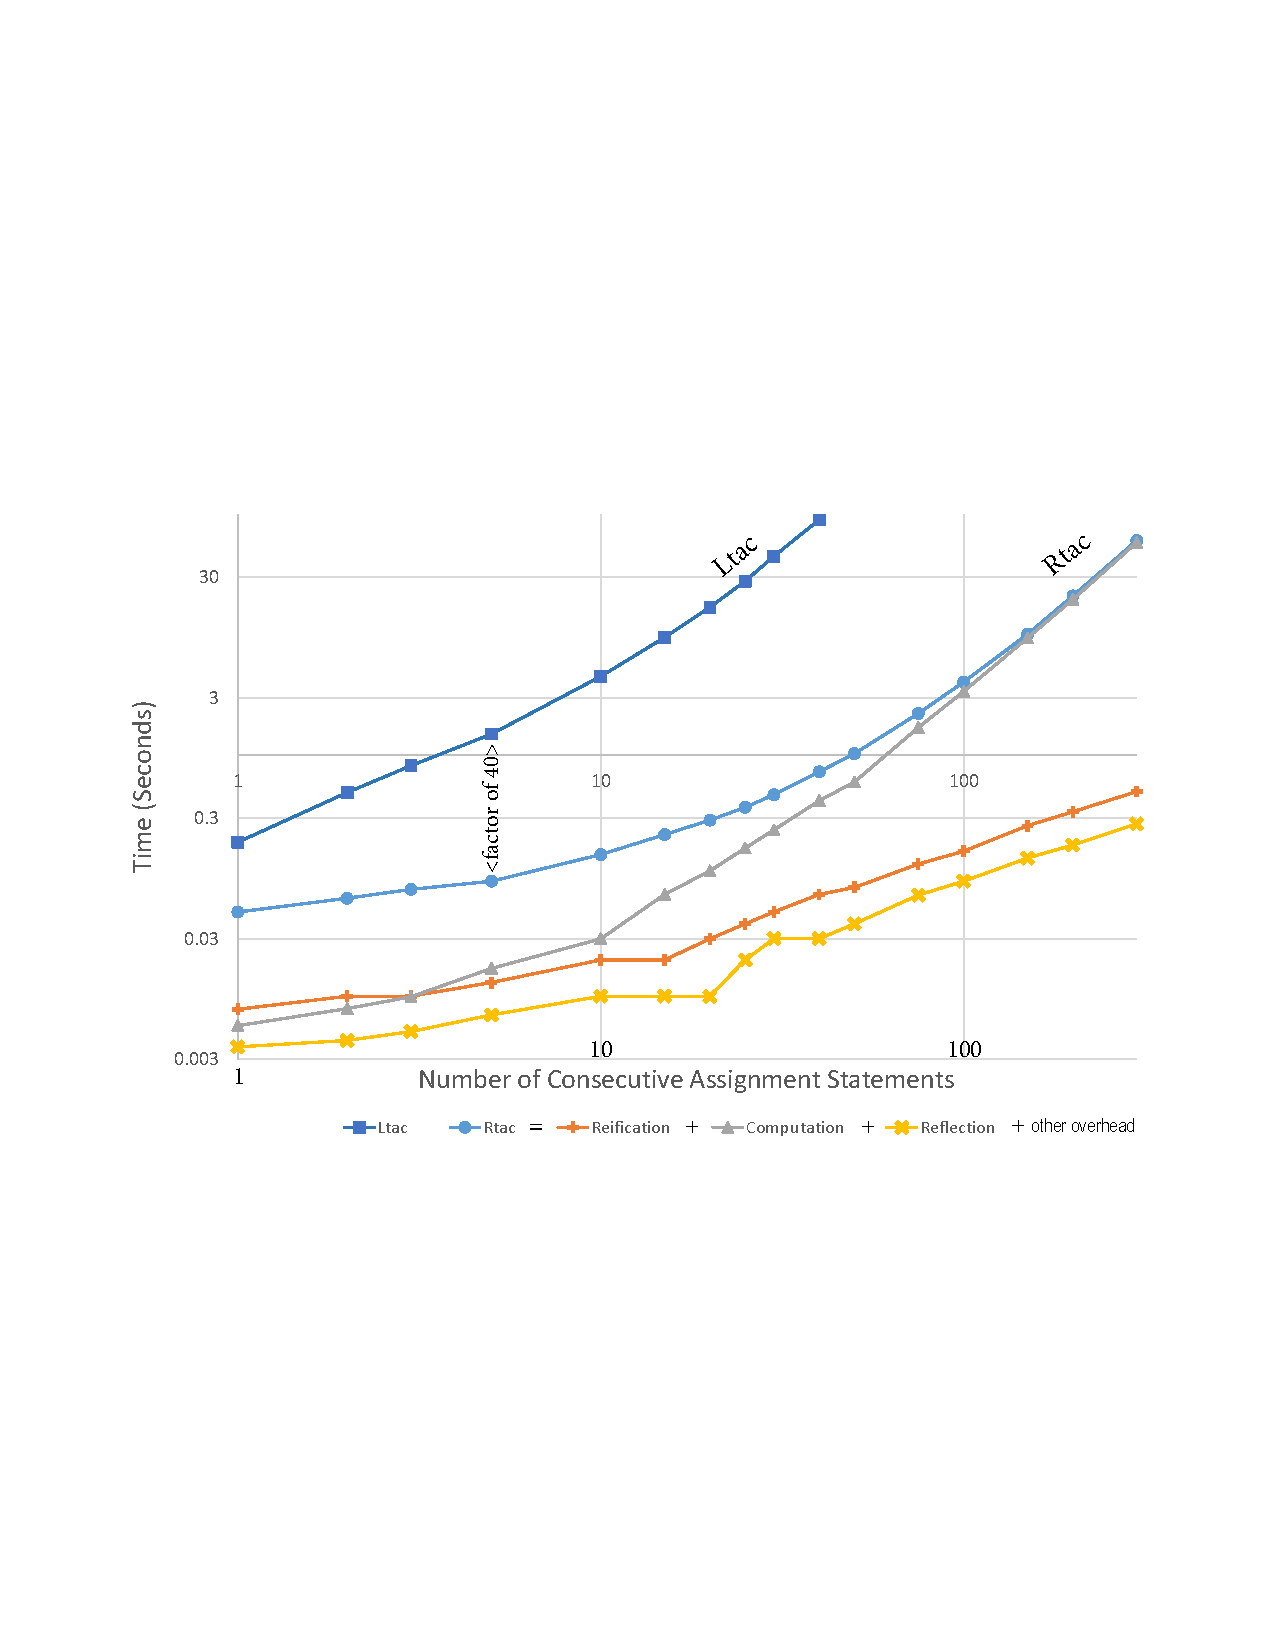
\includegraphics[width=\textwidth]{chart.pdf}
\vspace{-4ex}
\caption{Run time of Ltac vs Rtac, for $n$ consecutive C statements (log-log scale).}
\label{fig:chart}
\vspace{-4ex}
\end{figure}

Each data point is the average of 10 consecutive runs on a modern
laptop.  The timing information was obtained by Braibant's Timing
plugin \cite{braibant:timing} The amount of memory on the laptop is
over 2 gigabytes, which is the maximum amount of memory that 32-bit
Coq can use. Because it is very difficult to get 64-bit Coq on all
platforms, we attempt to write tactics that can operate within the
lower memory bounds.

Although this is a synthetic test, we consider it a lower bound on the
performance increase we will see in the process of a real proof. This
is because numerous other tests indicate that for non-addressed
variable assignments the size of the precondition has the predominant
effect on the run-time, rather than the meaning of the
precondition. This follows from what we would expect. The computation
that we need to do in both real and synthetic cases is almost all
getting and setting from efficient tree maps, where get and set take
$\log(n)$ time (where $n$ is the largest index in the domain of the
map). Our program input will be
compiled by CompCert, and CompCert uses small indices. The remainder
of the operations that RTac does are linear (or slower) unifications
between lemmas and proof goals, as well as linear (or slower) rewrites
by proved equalities. Repeated linear operations are what lead to the
$n^{2.5}$ operation we observe in the chart above, not repeated
$\log(n)$ gets and sets.

The chart shows that there 
is a speedup of (typically) 40$\times$ (e.g., running $n\! = \! 8$ consecutive
C-program statements). 
Speedup improves with scale: $n\! =\! 50$ 
steps in Ltac takes over 2 minutes, while
the same number of steps in Rtac takes only .9 seconds, running almost 150$\times$ faster! 
Even for $n\!=\!1$ there is a 4$\times$ speedup.
This greatly improves interactivity of the logic. In general it
seems that growth of time relative to the number of program steps is
quadratic. Our benchmark that uses more complex preconditions
scales even better (not shown in a graph),
with 74$\times$ speedup at $n\! = \!10$.


The \emph{computation} curve, at the upper end, clearly
shows a time complexity of $n^{2.5}$.
This time complexity is roughly what we expect,
because (in this example) the
precondition grows linearly with the number of steps,
and each step has proof operations at least proportional to the size
of the precondition.

On a real-life example, a loop-body from OpenSSL's SHA
function\footnote{The second loop body in the
  \lstinline{sha256_block_data_order} function of the cited paper
  \cite{appel15:sha}; there are 850 nodes in the loop body's abstract
  syntax tree.}  takes 336 seconds to verify in our Ltac
\lstinline{forward} tactic; \lstinline|rforward| takes only 12
seconds---a 28$\times$ speedup. The sequence includes 13
local-variable assignments, 5 loads, and 1 store, several of which
contain huge mathematical expressions (resulting from macro-expansion
in the C source code). The assertions in that example are large, with
many local-variable and spatial conjuncts.

Unfortunately, after Rtac has efficiently computed a proof, Coq's
\lstinline|Qed| blows up, taking minutes in some cases.  Qed blowups
tend to occur when Coq cannot find an efficient $\beta\eta$-conversion
sequence to prove an equality (even if the tactic script demonstrated
one).  Performance measurements in this section (for both Ltac and
Rtac) do not include Qed times; the Ltac Qed times are larger than the
Rtac Qed times, but both are terrible (e.g., 815 and 615 seconds,
respectively, for the SHA loop-body example).


\chapter{Conclusion}

\bibliographystyle{plain}
\bibliography{appel.bib}

\end{document}

